\documentclass[11pt]{article}

\usepackage[margin=1in]{geometry}
\usepackage{amsmath,amssymb,amsthm}
\usepackage{graphicx}
\usepackage{booktabs}
\usepackage{listings}
\usepackage{xcolor}
\usepackage{url}
\usepackage[hidelinks]{hyperref}
\usepackage{caption}
\usepackage{pgfplots}
\pgfplotsset{compat=1.18}

% Categorical slots 1-3 of the validated default palette (light surface),
% checked with the data-viz validator on the adjacent and all-pairs lists:
%   ALL CHECKS PASS; serC carries a contrast WARN, relieved by the direct
%   labels on every series and by the tables in the body.
\definecolor{serAc}{HTML}{2A78D6}
\definecolor{serBc}{HTML}{EB6834}
\definecolor{serCc}{HTML}{1BAF7A}
\definecolor{inkc}{HTML}{0B0B0B}
\definecolor{inktwoc}{HTML}{52514E}
\definecolor{gridgrayc}{HTML}{D8D7D2}
\tikzset{
  serA/.style={color=serAc, mark options={fill=serAc, draw=serAc}},
  serB/.style={color=serBc, mark options={fill=serBc, draw=serBc}},
  serC/.style={color=serCc, mark options={fill=serCc, draw=serCc}},
}
\colorlet{ink}{inkc}
\colorlet{inktwo}{inktwoc}
\colorlet{gridgray}{gridgrayc}

\lstset{
  basicstyle=\ttfamily\scriptsize,
  columns=fullflexible,
  keepspaces=true,
  breaklines=true,
  frame=single,
  framesep=3pt,
  rulecolor=\color{gray!50},
  backgroundcolor=\color{gray!5},
  showstringspaces=false,
}

\newtheorem{definition}{Definition}
\newtheorem{proposition}{Proposition}
\newtheorem{remark}{Remark}

\newcommand{\R}{\mathbb{R}}
\newcommand{\VD}{\mathrm{VD}}
\newcommand{\Arr}{\mathcal{A}}

\title{Vertical Decomposition of an Arrangement of Planes in $\R^3$:\\
An Exact Sweep-Based Implementation}

\author{Hayim Shaul\footnote{written using AI tools}}

\date{\today}

\begin{document}
\maketitle

\begin{abstract}
The vertical decomposition of an arrangement of surfaces refines every cell of
the arrangement into constant-complexity pseudo-prisms, and is the standard
device for turning arrangements of curved or high-dimensional objects into
objects that can be stored, located in, and searched.  We describe \texttt{vd3d},
an open-source implementation of the vertical decomposition of an arrangement
of $n$ planes in $\R^3$.  The implementation follows a sweep in the $z$
direction: it maintains the two-dimensional vertical (trapezoidal)
decomposition of the horizontal slice of the arrangement, and grows
three-dimensional prisms between consecutive combinatorial changes of that
slice.  Two event types drive the sweep --- triple intersections of input
planes, and \emph{vertical alignments}, at which two slice vertices acquire a
common $x$-coordinate and their trapezoidal walls collide.  All predicates and
constructions are evaluated in exact rational arithmetic, so the combinatorial
output is determined by the input and not by a floating-point tolerance.

We also describe a second, standalone construction in the same codebase, which
decomposes only the region below the \emph{lower envelope} of the planes.  It
dualizes each plane to a point, reads the envelope off the lower convex hull,
and decomposes the resulting minimization diagram directly.  Because the
envelope of $n$ planes bounds an intersection of $n$ halfspaces, this part of
the decomposition has $\Theta(n)$ rather than $\Theta(n^3)$ cells, and the
construction is some three orders of magnitude faster than the sweep at $n = 7$.
Experiments at $n \le 96$, together with a structured family built from the
Voronoi lifting for which the $\Theta(n)$ bound is attained, show that on random
input the envelope is drastically smaller than the bound --- six or seven planes
of 96 reach it --- and also expose a defect: the implementation's merge step
never fires on any instance we tried, so it emits a slab decomposition rather
than a trapezoidal map, with an over-refinement factor that grows with $n$.
Comparing the two exposes a definitional subtlety that the shared cell type
hides: they recurse in opposite order and therefore produce genuinely different
cells, with differently oriented walls, for the same input.

We describe both algorithms, the module structure of the implementation
($\approx 7.9$k lines of kernel code, $\approx 6.2$k lines of visualisation, and
$\approx 4.6$k lines of tests and oracles), and the verification architecture:
enforced invariants, brute-force oracles for every non-trivial sub-procedure,
differential testing of the incremental sweep against a from-scratch
recomputation at every event, and float-versus-exact cross-checking for the
envelope path.  We then report execution examples and benchmarks on random
instances with $n \le 8$ planes.  Measured running
time grows as roughly $n^{8}$, which we attribute not to the $\Theta(n^3)$
output size but to the per-event from-scratch recomputation of the slice
decomposition that the current implementation retains as a correctness oracle.
Finally we report a robustness evaluation.  On random instances $29\%$ of
reference-path sweep runs abort, and we trace that entire failure class to a single
scale-inconsistent comparison in the half-edge ordering at infinity: with a
one-line repair, all 160 instances of an independent scan complete.  A second,
smaller class is the differential assertion itself firing when the incremental
slice update disagrees with the recomputation at a group of simultaneous
events --- a correctness gap that the architecture detects rather than
conceals.  The envelope construction, which is shorter and touches neither
component, completed on every instance we ran.  Stressing it against Qhull over
five decades of coefficient magnitude produced disagreements only at the
\emph{narrowest} range, where inputs are degenerate rather than easy, and there
the exactly computed answer is the less useful of the two.
\end{abstract}

\tableofcontents

\section{Introduction}

An \emph{arrangement} $\Arr(P)$ of a set $P$ of $n$ planes in $\R^3$ is the
subdivision of space induced by those planes into vertices, edges,
two-dimensional faces, and open three-dimensional cells.  Arrangements are the
common substrate of a large part of computational geometry: motion planning,
visibility, Voronoi diagrams, range searching, and geometric optimisation all
reduce, at some level, to constructing or searching an arrangement
\cite{halperin-sharir-handbook,agarwal-sharir-handbook,edelsbrunner-book}.

A cell of an arrangement of planes is a convex polyhedron, but it may have
arbitrarily many facets, and in an arrangement of general surfaces a cell need
not even be simply connected.  The \emph{vertical decomposition} is the
standard remedy: each cell is cut by vertical walls into sub-cells of constant
descriptive complexity, so that the whole arrangement becomes a collection of
combinatorially simple pieces.  In the plane this is the familiar trapezoidal
map \cite{seidel-trapezoid,mulmuley}; in $\R^3$ and above it is the
decomposition of Chazelle, Edelsbrunner, Guibas and Sharir
\cite{chazelle-stratification}, which underlies the singly-exponential
stratification of semi-algebraic sets and, in its combinatorial form, the
best-known bounds for many substructure problems
\cite{tagansky,deberg-guibas-halperin,guibas-halperin-matousek-sharir,koltun}.

This paper describes \texttt{vd3d}, an implementation of the vertical
decomposition of an arrangement of planes in $\R^3$.  The implementation makes
four choices that distinguish it from a textbook exercise:

\begin{enumerate}
\item \textbf{A sweep formulation.}  Rather than constructing the arrangement
  and then decomposing each cell, the algorithm sweeps a horizontal plane
  $H(z)$ upward and maintains the two-dimensional vertical decomposition of the
  slice $\Arr(P) \cap H(z)$.  A three-dimensional prism is exactly a
  two-dimensional trapezoid extruded over a maximal $z$-interval during which
  the slice decomposition does not change combinatorially.  This reduces the
  three-dimensional problem to a sequence of local updates of a planar
  trapezoidal map.
\item \textbf{Exact arithmetic throughout.}  Every coordinate and coefficient
  in the geometric kernel is a Python \texttt{fractions.Fraction}.  Floating
  point is confined to the visualisation layer by an enforced architectural
  rule.  This places the implementation squarely in the exact geometric
  computation paradigm \cite{yap-egc,kettner-classroom}, at a cost in speed
  that we measure.
\item \textbf{Verification as a first-class artefact.}  Every non-trivial
  sub-procedure is accompanied by a brute-force oracle, and the incremental
  sweep is differentially tested at every event against a from-scratch
  recomputation of the slice.  The test suite is roughly as large as the
  computational kernel.
\item \textbf{A specialised construction alongside the general one.}  The cells
  below the lower envelope of the planes are built separately, by duality and
  convex hull rather than by sweeping.  That part of the decomposition has
  linear rather than cubic size, and isolating it turns out to matter for both
  speed and robustness.
\end{enumerate}

Section~\ref{sec:background} gives the academic background.
Section~\ref{sec:problem} fixes conventions and states precisely what the
implementation computes.  Section~\ref{sec:algorithm} describes the sweep and
Section~\ref{sec:hypograph} the lower-envelope construction;
Section~\ref{sec:implementation} describes the code.
Section~\ref{sec:examples} gives worked execution examples,
Section~\ref{sec:benchmarks} benchmarks, and Section~\ref{sec:robustness} an
honest robustness evaluation including a diagnosed defect.

\section{Background}
\label{sec:background}

\subsection{Arrangements of hyperplanes}

For $n$ hyperplanes in $\R^d$ in general position, the arrangement has
$\Theta(n^d)$ faces of all dimensions, and it can be constructed in
$\Theta(n^d)$ time by the incremental algorithm of Edelsbrunner, O'Rourke and
Seidel \cite{eos86}, which is optimal.  In $\R^3$ this is $\Theta(n^3)$: an
arrangement of $n$ planes in general position has $\binom{n}{3}$ vertices,
$\binom{n}{2}(n-1) = n(n-1)^2/2$ edges (each of the $\binom{n}{2}$ intersection
lines is cut into $n-1$ pieces by the remaining $n-2$ planes), and
$\sum_{i=0}^{3}\binom{n}{i}$ full-dimensional cells.  The standard references are Edelsbrunner's monograph
\cite{edelsbrunner-book} and the arrangements chapters of the two handbooks
\cite{halperin-sharir-handbook,agarwal-sharir-handbook}.

The difficulty that motivates vertical decomposition is not the total size of
the arrangement but the complexity of an \emph{individual} cell.  A single cell
of an arrangement of $n$ planes can have $\Theta(n)$ facets; for arrangements
of surfaces the situation is worse, since cells may be non-convex and of
unbounded topological complexity.  Algorithms that want to walk, locate in, or
point-query a cell need cells of bounded description size.

\subsection{Vertical decomposition}

Let $\Arr$ be an arrangement of surfaces in $\R^d$.  The vertical decomposition
$\VD(\Arr)$ is obtained by erecting, from every boundary feature of every cell,
a maximal ``vertical'' wall in the $x_d$ direction, recursing on the resulting
cross-sections in dimension $d-1$, and stopping when the pieces have constant
descriptive complexity.  In the plane the construction collapses to the
trapezoidal map: from every vertex of the arrangement shoot two vertical rays
until they hit another edge, producing $O(n^2)$ trapezoids, each with at most
two vertical sides and at most two non-vertical sides
\cite{seidel-trapezoid,mulmuley,deberg-book}.

Chazelle, Edelsbrunner, Guibas and Sharir \cite{chazelle-stratification}
introduced the general construction and proved a bound of $O(n^{2d-3})$ on its
size for arrangements of well-behaved surfaces --- singly exponential in $d$,
which is what makes it usable in the stratification of semi-algebraic sets, in
contrast to the doubly exponential cylindrical algebraic decomposition
\cite{collins-cad,schwartz-sharir}.  Improved bounds followed for special
cases: de Berg, Guibas and Halperin \cite{deberg-guibas-halperin} for triangles
in $3$-space, Tagansky \cite{tagansky} by a general charging technique, Guibas,
Halperin, Matou\v{s}ek and Sharir \cite{guibas-halperin-matousek-sharir} for
hyperplanes in $\R^4$, and Koltun \cite{koltun}, who established an almost
tight $O(n^{2d-4+\varepsilon})$ bound in four dimensions and above.

For the case treated here --- $n$ planes in $\R^3$ --- the situation is
comparatively simple.  The arrangement has $\Theta(n^3)$ complexity and so does
its vertical decomposition: each of the $\Theta(n^3)$ cells is convex with
$O(n)$ facets, and the decomposition of a convex polyhedron with $k$ facets
into vertical prisms produces $O(k^2)$ pieces, which sums to $O(n^3)$ over the
whole arrangement by the zone theorem.  The interest of the three-dimensional
case is therefore not its asymptotics but its role as the smallest setting in
which the full recursive structure of the decomposition --- walls in $x_3$,
then walls in $x_2$ inside each cross-section --- actually appears, and in which
the degeneracies that dominate implementation effort can be exhibited and
tested.

\subsection{Exact geometric computation}

Geometric algorithms are combinatorial algorithms driven by numerical
predicates.  When those predicates are evaluated in floating point, the
combinatorial decisions can become mutually inconsistent, and the algorithm can
produce structurally invalid output or fail to terminate --- a failure mode
documented at length by Kettner, Mehlhorn, Pion, Schirra and Yap
\cite{kettner-classroom}.  The exact geometric computation paradigm
\cite{yap-egc} responds by guaranteeing that every predicate is evaluated to
its true sign, either with exact arithmetic (LEDA \cite{leda}, CGAL
\cite{cgal}), with adaptive filters and exact fallbacks
\cite{fortune-vanwyk,shewchuk-predicates}, or, as here, by simply computing in
$\mathbb{Q}$.

Vertical decomposition is a construction, not merely a predicate evaluation:
its walls are new geometric objects whose coordinates are rational functions of
the input.  A floating-point implementation would therefore have to contend not
only with predicate errors but with constructed-object drift.  Working in
$\mathbb{Q}$ removes both problems and makes the output a deterministic
function of the input, at the price of coefficient growth, which we measure in
Section~\ref{sec:benchmarks}.

\section{Problem statement and conventions}
\label{sec:problem}

\subsection{Input}

The input is a set $P = \{P_1,\dots,P_n\}$ of planes, each given by exact
rational coefficients in the form
\[
  P_i:\quad a_i x + b_i y + c_i z + d_i = 0,
  \qquad (a_i,b_i,c_i) \neq (0,0,0).
\]
Coefficients are stored as given and are never normalised.  The residual
$P_i(p) = a_i p_x + b_i p_y + c_i p_z + d_i$ carries the orientation: $P_i(p) >
0$ on the side the normal points to, $P_i(p) < 0$ on the other.

\subsection{Sweep axis and two meanings of ``vertical''}

The sweep coordinate is $z$.  At a fixed height $z_0$ the horizontal plane
$H(z_0) = \{(x,y,z_0)\}$ cuts each input plane $P_i$ in the line
\begin{equation}
  \ell_i(z_0):\quad a_i x + b_i y + (c_i z_0 + d_i) = 0 ,
  \label{eq:slice}
\end{equation}
which is well defined unless $a_i = b_i = 0$ (a horizontal input plane, which
contributes no slice line and is dropped).

The word ``vertical'' is used at two levels, and the distinction matters:

\begin{itemize}
\item \textbf{2D vertical} means parallel to the $y$-axis, i.e.\ $x =
  \mathrm{const}$.  The walls of the two-dimensional decomposition of a slice
  are 2D-vertical.
\item \textbf{3D vertical} refers to the walls of the three-dimensional cells.
  Each such wall is the surface swept by one 2D-vertical wall of the slice as
  $z$ varies.  Since a 2D wall sits at $x = x_L(z)$ for some intersection line
  $L$, and $x_L$ is affine in $z$ (equation \eqref{eq:xofz} in Section~\ref{sec:algorithm}), the swept surface is
  the $y$-parallel plane
  \[
    x - \alpha z - \beta = 0, \qquad \alpha = d_x/d_z,\ \ \beta = x_0 - z_0\alpha ,
  \]
  which has no $y$ term.  When $\alpha = 0$ the wall is also parallel to the
  $z$-axis and degenerates to $x = \mathrm{const}$; otherwise it tilts.  This is
  worth stating explicitly because the project's own
  \texttt{docs/conventions.md} describes a 3D vertical wall as ``a plane
  parallel to the $z$-axis'', which is the $\alpha = 0$ special case rather than
  the general one.  The code emits the general form: in the three-plane example
  of Section~\ref{sec:examples}, 8 of the 20 emitted walls are $x = 1$ and the
  other 12 are $x + z - 4 = 0$, and on a random five-plane instance all 159
  emitted walls tilt.
\end{itemize}

\subsection{Output}

A cell of the output is a trapezoid of the slice decomposition extruded over a
maximal $z$-interval on which that trapezoid persists.  Concretely:

\begin{definition}[3D cell]
A cell is a (possibly unbounded) prism described by
\begin{itemize}
\item a \emph{floor}: at most one input plane, or none (unbounded);
\item a \emph{ceiling}: at most one input plane, or none (unbounded);
\item at most four \emph{vertical walls}, each a $y$-parallel plane
  $x - \alpha z - \beta = 0$;
\item a $z$-extent $(z_{\mathrm{lo}}, z_{\mathrm{hi}})$, with $\pm\infty$
  allowed.
\end{itemize}
\end{definition}

\begin{remark}
The names \emph{floor} and \emph{ceiling} are inherited from the design
document and are slightly misleading: they are the lower and upper supporting
planes of the underlying \emph{trapezoid}, so they bound the cell in the $y$
direction of the slice, not in $z$.  The bounds in $z$ are carried separately as
$z_{\mathrm{lo}}$ and $z_{\mathrm{hi}}$.  The invariant the code enforces is
``at most one floor plane, at most one ceiling plane, at most four vertical
walls, and $z_{\mathrm{lo}} < z_{\mathrm{hi}}$ for bounded cells''; the bound of
four is the general vertical-decomposition bound, while this construction in
fact produces at most two walls per cell, since a trapezoid has at most one
wall on each side.
\end{remark}

\subsection{General position, and its relaxation}

The first version of the algorithm assumed: no two planes parallel; no four
planes through a common point; no two independent events at the same $z$; no
vertical input plane; no vertical intersection line.  The current
implementation relaxes all but the last of these.  Events that share a height
are processed as one atomic \emph{event group}; query lines are allowed to pass
through arrangement vertices or to overlap an arrangement edge; four planes
through a point and vertical input planes ($c = 0$) are covered by fixtures.
Horizontal intersection lines ($dz = 0$) are still skipped when generating
alignment events, and coincident input planes are treated as parallel and
ignored.  Passing \verb|require_general_position=True| restores the strict
behaviour and raises on a simultaneous group.

\section{The algorithm}
\label{sec:algorithm}

\subsection{Overview}

\begin{enumerate}
\item Compute all pairwise intersection lines $L_{ij} = P_i \cap P_j$, skipping
  parallel pairs.
\item Generate all sweep events and sort them by $z$.
\item Choose a height $z_0$ strictly below every event, and compute the
  two-dimensional vertical decomposition of the slice there from scratch.  Open
  one 3D cell per 2D trapezoid, with $z_{\mathrm{lo}} = -\infty$.
\item For each event group in increasing $z$: compute the slice decomposition
  just below and just above, match cells across the event, close the 3D cells
  whose 2D trapezoid disappears, continue those that persist, and open new ones.
\item After the last event close all remaining cells at $z = +\infty$.
\end{enumerate}

\subsection{Events}

The combinatorial structure of the slice decomposition changes at exactly two
kinds of heights.

\paragraph{Triple intersections.}
Three planes $P_i, P_j, P_k$ meet in a point $p$ whenever the $3 \times 3$
system
\[
  \begin{pmatrix} a_i & b_i & c_i \\ a_j & b_j & c_j \\ a_k & b_k & c_k
  \end{pmatrix}
  \begin{pmatrix} x \\ y \\ z \end{pmatrix}
  = \begin{pmatrix} -d_i \\ -d_j \\ -d_k \end{pmatrix}
\]
is non-singular.  At $z = p_z$ the three slice lines $\ell_i, \ell_j, \ell_k$
become concurrent; just below and just above they bound a small triangle.  The
number of such events is at most $\binom{n}{3}$, and exactly $\binom{n}{3}$ in
general position.

\paragraph{Vertical alignments.}
This is the event type specific to the vertical decomposition, and the one that
does not exist in a plain arrangement sweep.  The walls of a two-dimensional
vertical decomposition are erected at the $x$-coordinates of the arrangement
vertices.  As $z$ varies, each arrangement vertex is the slice of an
intersection line $L$, and its $x$-coordinate traces the affine function
\begin{equation}
  x_L(z) = \frac{d_x}{d_z}\, z + \Bigl(x_0 - z_0 \frac{d_x}{d_z}\Bigr),
  \label{eq:xofz}
\end{equation}
where $(d_x,d_y,d_z)$ is the direction of $L$ and $(x_0,y_0,z_0)$ a point on
it.  Two intersection lines $L_1, L_2$ \emph{align} at the height $z$ solving
$x_{L_1}(z) = x_{L_2}(z)$, provided that at that height the two slice vertices
are distinct and the open vertical segment joining them meets no other
arrangement feature.  At such a height two walls of the decomposition become
collinear, trapezoids merge or split, and the 3D cell structure changes even
though the underlying arrangement does not.

\subsection{Detecting alignments through a wall zone}

Enumerating all $O(n^4)$ pairs of intersection lines and testing visibility is
correct but wasteful, and the implementation keeps that enumeration only as an
oracle.  The production path localises the search using a zone computation.

For an intersection line $L$ with $d_z \neq 0$, define its \emph{vertical
wall} $W(L)$: the unique $y$-parallel plane containing $L$,
\[
  W(L):\quad x - \alpha z - \beta = 0, \qquad
  \alpha = \frac{d_x}{d_z},\ \ \beta = x_0 - z_0\alpha .
\]
$W(L)$ is exactly the surface swept by the 2D-vertical wall of $L$'s slice
vertex as $z$ varies.  Substituting $x = \alpha z + \beta$ into each input plane
gives a two-dimensional line arrangement in the wall frame $(z, y)$, in which
$L$ itself is one of the lines.  The candidates for alignment with $L$ are then
precisely the vertices of the faces incident to $L$ that do \emph{not} lie on
$L$ --- the ``opposite vertices'' of the supporting-line zone of $L$
(Figure~\ref{fig:showsweep} shows the geometry in slice form).  Each surviving
candidate is validated against the visibility predicate.  Each geometric event
is discovered from both of its walls and deduplicated by the canonical key
$(\text{type}, z, \text{sorted line ids})$.

\subsection{Matching cells across an event}

Let $\VD^-$ and $\VD^+$ be the slice decompositions at $z \mp \varepsilon$.  A
trapezoid $C^- \in \VD^-$ continues as the same 3D cell as $C^+ \in \VD^+$ when

\begin{enumerate}
\item the representative point of each lies in the open interior of the other, and
\item their lower and upper supporting plane identifiers agree.
\end{enumerate}

Far from the event this matching is a bijection; the unmatched remainder is
exactly the event neighbourhood.  Between events the set of active cells is
keyed by a \emph{cell signature}: the supporting planes, the boundedness of the
left and right walls, and the source planes of the vertices carrying those
walls.  Signatures are unique within a slice and constant on an open
$z$-interval, which is what allows a 3D cell to be identified across a whole
interval without storing geometry.

The offset $\varepsilon$ is taken to be $1/100$, or half the gap to the nearest
\emph{distinct} event height when that is smaller.  Because the arithmetic is
exact, $\varepsilon$ is a genuine rational displacement and not a tolerance:
correctness requires only that no other event lies in $(z-\varepsilon,
z+\varepsilon)$.

\subsection{The local update}

A from-scratch recomputation of $\VD^+$ at every event is correct but costs
$\Theta(\text{slice size})$ per event.  The incremental path instead rebuilds
only the affected strip:

\begin{enumerate}
\item Identify the event's defining vertices by the sorted plane identifiers of
  the lines through them: for a triple, the three pairwise intersections; for
  an alignment, the two slice vertices of the two intersection lines.
\item Take the \emph{$x$-window}: the closed interval spanned by those vertices'
  $x$-coordinates at $z^-$ and at $z^+$.
\item Every arrangement vertex in that window is local; its $\pm y$ rays are
  re-shot on the after-slice.  Every vertex outside keeps its before-event
  first-hit combinatorics --- which supporting plane its ray hits --- and only
  the geometry of that hit is re-evaluated at the new height.
\item Rebuild the trapezoids from the resulting walls.
\end{enumerate}

For a group of simultaneous events the windows are unioned into one strip,
because a vertex sitting between two same-height features still has to be
re-shot.

\subsection{Complexity}
\label{sec:complexity}

We separate the complexity of the \emph{problem} from the complexity of the
\emph{current implementation}, because the two differ substantially.

\paragraph{Output size.}
The decomposition has $\Theta(n^3)$ cells, matching the arrangement.  Each
slice decomposition has $O(n^2)$ trapezoids, and the sweep passes through
$O(n^3)$ events (at most $\binom{n}{3}$ triples, and $O(n^3)$ visible
alignments, since each visible alignment corresponds to a wall collision and is
therefore charged to a cell of the output).

\paragraph{Event generation.}
Triple generation is $\Theta(n^3)$ determinant evaluations.  Alignment
generation, as implemented, iterates over the $O(n^2)$ intersection lines and
for each one builds a complete line arrangement of $n$ wall traces and its
supporting-line zone.  With an $A(n)$-cost arrangement construction this is
$O(n^2 A(n))$.

\paragraph{Per-event work.}
Both paths recompute \emph{both} slices from scratch at every event group:
instrumenting \texttt{compute\_vd\_at\_z} shows exactly $2.00$ calls per event
group, and that figure is identical with \verb|incremental=True| and
\verb|incremental=False|.  The incremental flag does not change how many slices
are built; it only changes which object becomes $\VD^+$.  The two calls have
different standing:

\begin{itemize}
\item $\VD^-$ is load-bearing on both paths.  It supplies the before-side
  geometry for \texttt{match\_cells}, the signature that looks up which active
  3D cell to end or continue, and the input to the incremental handler.
\item $\VD^+$ is load-bearing only on the reference path, where it \emph{is}
  the after-slice.  On the incremental path the after-slice comes from the local
  update, and the recomputed $\VD^+$ is used solely for the
  \texttt{same\_combinatorics} assertion (Section~\ref{sec:verification}).
\end{itemize}

The incremental path is therefore strictly more expensive than the reference
path today --- same two recomputations, plus the local update, plus the
comparison.  Its value is as a validated algorithm, not yet as a speedup.

\begin{remark}
\label{rem:current-vd}
The sweep threads a \texttt{current\_vd} through the whole loop --- nominally
the maintained sweep-line structure --- but it is never used as an input.  Its
only consumer is the guard
\verb|same_combinatorics(current_vd, vd_before)|, which asserts that the
structure carried forward agrees with the slice just recomputed at $z^-$.  So
the algorithm as written is not maintaining a swept decomposition in the
incremental sense: it re-derives $\VD^-$ from scratch at every event while
holding the previous event's output alongside it as a check.  This is the
single largest gap between the implementation and the algorithm it implements,
and it is invisible in the output, which is correct either way.
\end{remark}

\paragraph{Constructed-coordinate growth.}
Every wall coordinate is a rational function of the input coefficients.  Bit
sizes grow along the chain \emph{plane $\to$ intersection line $\to$ wall $\to$
alignment height $\to$ slice at $z \pm \varepsilon$ $\to$ trapezoid
representative}.  Measuring the trapezoid representatives of the slices taken
around events, on instances whose input coefficients are single-digit integers,
gives a median denominator of about $2\,000$ at $n = 4$ and about $5\,000$ at
$n = 6$, with the largest observed exceeding $1.9 \times 10^{6}$.  Every
comparison in the sweep is then a comparison of rationals of that size.  This is
the price of exactness, and it is one of the contributions to the constants in
the measured running times.

\section{A second construction: the hypograph of the lower envelope}
\label{sec:hypograph}

The sweep of Section~\ref{sec:algorithm} produces the whole decomposition.  A
separate package, \texttt{vd3d.lower\_envelope}, produces only the part of it
that lies under the \emph{lower envelope} of the planes --- the cells that are
unbounded downwards --- and does so without sweeping at all.  The two
constructions are worth presenting together because the second is cheap,
robust and almost trivially correct where the first is expensive and fragile,
and because comparing them exposes a definitional subtlety that the shared data
type hides.

\subsection{Duality and the lower envelope}

Write each non-vertical plane ($c \neq 0$) in graph form
\[
  z = f_i(x,y) = A_i x + B_i y + C_i,
  \qquad A_i = -\tfrac{a_i}{c_i},\ \ B_i = -\tfrac{b_i}{c_i},\ \ C_i = -\tfrac{d_i}{c_i},
\]
and map it to the dual point $p_i = (A_i, B_i, C_i)$.  The lower envelope
\[
  f(x,y) = \min_i \langle p_i, (x, y, 1)\rangle
\]
is then read off the \emph{lower convex hull} of the dual point set, under the
classical correspondence

\begin{center}
\begin{tabular}{ll}
\toprule
lower hull of $\{p_i\}$ & lower envelope of $\{P_i\}$ \\
\midrule
vertex $p_i$            & a face (plane $i$ is lowest there) \\
edge $(p_i, p_j)$       & an edge (planes $i$ and $j$ meet) \\
facet $(p_i,p_j,p_k)$   & a vertex (triple intersection point) \\
\bottomrule
\end{tabular}
\end{center}

\begin{proposition}[why this part is cheap]
\label{prop:envelope-linear}
The region below the lower envelope is $\bigcap_i \{z \le f_i(x,y)\}$, an
intersection of $n$ halfspaces, so its boundary is a convex polyhedral surface
with at most $n$ faces and therefore $O(n)$ vertices and edges in total.  Its
projection to the $xy$-plane --- the minimization diagram --- is a convex planar
subdivision with $O(n)$ features, so its trapezoidal decomposition has $O(n)$
cells.
\end{proposition}

So the trapezoidal map of the hypograph carries $\Theta(n)$ cells, against
$\Theta(n^3)$ for the whole decomposition --- which is why this part of the
problem is cheap.  Two caveats, both established experimentally in
Section~\ref{sec:benchmarks} and both worth flagging here.  On random input the
envelope is far smaller than the bound: only six or seven of 96 planes reach it
(Section~\ref{sec:bench-env-scaling}).  And the implementation does not attain
the bound even when the envelope does, because its merge step never fires and
it emits a slab decomposition instead of a trapezoidal map
(Section~\ref{sec:bench-merge}).  The proposition bounds the problem, not this
code.

\subsection{Pipeline}

The package runs four stages, in two matched pairs:

\begin{enumerate}
\item \textbf{Float envelope} (\texttt{envelope\_float.py}): dualize, call
  \texttt{scipy.spatial.ConvexHull} (Qhull), and keep the facets whose outward
  normal has negative $z$.
\item \textbf{Float hypograph VD} (\texttt{vd\_float.py}): decompose the
  minimization diagram into $y$-parallel trapezoids and lift each to a
  \texttt{Cell3D}.
\item \textbf{Exact envelope} (\texttt{dual.py}, \texttt{hull.py},
  \texttt{envelope.py}): the same duality over \texttt{Fraction}.
  \texttt{lower\_hull\_facets} is a frank brute force --- for every triple
  $(i,j,k)$ it orients the supporting plane so that $n_z < 0$ and checks that
  every other dual point lies on the inward side, which is $O(n^4)$ and which
  the source comments acknowledge as adequate for the sizes targeted.
\item \textbf{Exact hypograph VD} (\texttt{vd.py}): the same trapezoid
  construction in exact arithmetic.
\end{enumerate}

The trapezoid construction mirrors the planar decomposition of
Section~\ref{sec:algorithm}: the $x$-coordinates of the envelope vertices cut
the plane into strips; inside a strip, \texttt{bands\_at\_x} evaluates the
one-dimensional lower envelope at a sample abscissa to get the $y$-bands; and
adjacent strip pieces with the same supporting plane and the same band are
merged unless a wall erected at an envelope vertex blocks them.  Each surviving
trapezoid is lifted by \texttt{trapezoid\_to\_cell3d} to
\verb|Cell3D(floor=None, ceiling=|$P_i$\verb|)|.

\subsection{The walls here are genuinely vertical}
\label{sec:hypograph-walls}

This construction resolves, in its own scope, the discrepancy noted in
Section~\ref{sec:problem}.  Its two wall constructors are
\[
  \texttt{\_wall\_plane\_x}:\ x - x_0 = 0,
  \qquad
  \texttt{\_wall\_plane\_y\_line}:\ -m x + y - b = 0,
\]
both with $c = 0$: they are parallel to the $z$-axis, which is what
\texttt{docs/conventions.md} says a 3D vertical wall is.  Counting the walls
actually emitted on \texttt{examples/three\_planes.txt}:

\begin{center}
\begin{tabular}{lrr}
\toprule
wall orientation & sweep & hypograph \\
\midrule
$x = \mathrm{const}$ (both $y$- and $z$-parallel) & 8 & 4 \\
$z$-parallel, not $x = \mathrm{const}$            & 0 & 4 \\
$y$-parallel, tilting with $z$                    & 12 & 0 \\
\bottomrule
\end{tabular}
\end{center}

\begin{remark}[the two packages decompose differently]
\label{rem:two-decompositions}
They share the \texttt{Cell3D} dataclass, and \verb|floor=None| means different
things in each.  In the hypograph package it means what it says: the cell
extends to $z = -\infty$.  In the sweep it means that the underlying trapezoid
has no lower supporting line, i.e.\ the cell is unbounded in $-y$ within its
slice --- which is compatible with being bounded below in $z$.  On
\texttt{examples/three\_planes.txt} the sweep reports six cells with
\verb|floor=None|, three of them with $z$-extent $(3, +\infty)$; the hypograph
VD reports four, all with unbounded extent.  The ceiling multisets differ too:
$P_1$ is the ceiling of two hypograph cells and of no \verb|floor=None| sweep
cell.

The clearest way to see it is to locate one point in both.  For
$p = (5,5,-20)$, which lies below the envelope:
\begin{center}
\begin{tabular}{lll}
\toprule
& ceiling & walls, $z$-extent \\
\midrule
sweep      & $x{+}y{+}z{-}6=0$ & $x-1=0$, $x+z-4=0$; \quad $z \in (-\infty, 3)$ \\
hypograph  & $x{+}y{+}z{-}6=0$ & $x-1=0$, $y-2=0$; \quad\ \ $z \in (-\infty, +\infty)$ \\
\bottomrule
\end{tabular}
\end{center}
Same ceiling plane, different walls, and the sweep cell carries a horizontal
cap at the event height $z = 3$ that the hypograph cell does not.  These are two
different decompositions of the same region, not two views of one.

The reason is the order of the recursion.  The textbook construction cuts in
$z$ first (giving each cell one floor and one ceiling surface and $z$-parallel
walls), then recurses in $y$ inside the $xy$-projection; that is what the
hypograph package does.  The sweep instead cuts in $y$ inside each horizontal
slice and gets its $z$ subdivision incidentally, from the event heights.  Both
yield cells of constant descriptive complexity, which is all the applications
need, but they are not the same cells and the two packages' outputs should not
be compared cell for cell.
\end{remark}

\subsection{Verification by cross-arithmetic}

The verification strategy here is different from the rest of the project, and
in one respect inverted.  Elsewhere a slow exact brute force is the oracle for a
fast exact algorithm.  Here the two implementations differ in their
\emph{arithmetic}: Qhull in double precision against the same duality in
$\mathbb{Q}$.  \texttt{compare\_envelopes\_float\_exact} checks that the active
plane sets, the facet sets and the edge sets agree exactly as combinatorial
objects, and that matched vertices agree to $10^{-8}$;
\texttt{compare\_hypograph\_float\_exact} checks cell counts, the multiset of
ceiling planes, and trapezoid $x$-boundaries to $10^{-5}$.  Over the 100 random
instances of Section~\ref{sec:bench-hypograph} there were no disagreements.

This catches a different class of bug from an exact oracle --- a predicate whose
exact sign is wrong in the same way in both paths would survive it --- so we
also ran an independent partition oracle, which the package's own test file does
not contain.  A point is below the envelope exactly when
$z < \min_i f_i(x,y)$; every such point off every cell boundary must lie in
exactly one open cell, and every point above the envelope in none.  On 21
instances ($n \le 6$) and roughly $63\,000$ exact rational sample points, there
were no gaps, no overlaps, and no spurious containments; it still passes on the
wider sampler up to $n = 32$ (Section~\ref{sec:bench-oracle}).  The scripts are
\texttt{paper/scripts/hypograph\_oracle.py} and
\texttt{paper/scripts/bench\_envelope\_scaling.py}.

A third check, available only on structured input, is stronger than either: on
the Voronoi lifting of Section~\ref{sec:bench-voronoi} the ceiling of a cell
must be the plane of the sample point's nearest site, which tests the whole
pipeline against an independently computed nearest neighbour rather than against
a second implementation of the same idea.  It passed on all $10\,500$ points
tried.

\begin{remark}
Our first version of that oracle reported coverage gaps.  They were an artefact:
the sample grid used small integer coordinates, which land exactly on diagram
edges and wall lines, where belonging to no \emph{open} cell is the correct
answer.  Sampling rationals with denominator $997$ instead, and classifying
boundary hits separately, removed every reported failure.  We mention it because
it is the characteristic hazard of testing an exact implementation: round
coordinates are precisely the degenerate ones.
\end{remark}

\subsection{Code size and architectural cost}

The package is 2\,000 lines across eight modules, plus 590 lines in four visualisation
modules, and it has its own CLI (\verb|python -m vd3d.lower_envelope|, with
\verb|--exact|, \verb|--vd| and \verb|--gui| flags).  It brings one real
architectural cost.  The rule that no kernel package may import floating-point
machinery, which Section~\ref{sec:implementation} describes as enforced, now
carries an exemption: \texttt{tests/unit/test\_architecture.py} skips files
named \verb|*_float.py| and \verb|__main__.py| under
\texttt{vd3d/lower\_envelope} when checking for \texttt{numpy},
\texttt{matplotlib} and \texttt{vd3d.viz} imports, and \texttt{scipy} is now a
declared dependency.  The exemption is narrow, deliberate and documented in the
test, and the exact modules of the package remain free of floating point; but
``no floating point in the kernel'' is now ``no floating point in the kernel
except in modules whose names end in \texttt{\_float}''.

\section{Implementation}
\label{sec:implementation}

\subsection{Module structure}

The library is written in Python ($\ge 3.11$).  The sweep kernel has no
third-party dependency at all; \texttt{matplotlib} is required only for
visualisation, \texttt{pytest} only for the tests, and \texttt{scipy} only by
the float reference modules of \texttt{lower\_envelope}
(Section~\ref{sec:hypograph}).  Table~\ref{tab:loc} gives the module breakdown.

\begin{table}[htbp]
\centering
\begin{tabular}{llrr}
\toprule
Package & Role & Files & Lines \\
\midrule
\texttt{vd3d/geometry}               & planes, lines, exact scalars, linear algebra & 10 & 600 \\
\texttt{vd3d/arrangement2d}          & DCEL of a 2D line arrangement                 & 8  & 932 \\
\texttt{vd3d/vertical\_decomposition}& trapezoidal map of a slice                    & 6  & 934 \\
\texttt{vd3d/zone}                   & zone of a query line, supporting-line zone    & 7  & 676 \\
\texttt{vd3d/events}                 & intersection lines, triples, alignments       & 11 & 967 \\
\texttt{vd3d/sweep}                  & sweep driver, matching, local update, location& 9  & 1143 \\
\texttt{vd3d/cells3d}                & 3D cell lifecycle and invariants              & 5  & 361 \\
\texttt{vd3d/lower\_envelope}        & dual hull + hypograph VD (float and exact)    & 8  & 2000 \\
\texttt{vd3d/cli.py}, \texttt{io.py} & command line and plane I/O                    & 3  & 302 \\
\midrule
\multicolumn{2}{l}{\emph{kernel subtotal}}                                           & 67 & 7915 \\
\texttt{vd3d/viz}                    & plotting, galleries, interactive viewers      & 34 & 6237 \\
\texttt{tests/}                      & unit tests, oracles, visual fixtures          & 42 & 4649 \\
\bottomrule
\end{tabular}
\caption{Module breakdown.  \texttt{lower\_envelope} is the standalone
hypograph construction of Section~\ref{sec:hypograph}; everything above it is
the sweep.  The visualisation layer is comparable in size to the kernel, and
the test and oracle code to either.}
\label{tab:loc}
\end{table}

Two architectural rules are enforced by a dedicated test
(\texttt{tests/unit/test\_architecture.py}):

\begin{itemize}
\item the two-dimensional packages (\texttt{arrangement2d},
  \texttt{vertical\_decomposition}, \texttt{zone}) must not import
  \texttt{events}, \texttt{sweep}, or \texttt{cells3d};
\item no kernel package may import \texttt{vd3d.viz}, \texttt{matplotlib} or
  \texttt{numpy}.
\end{itemize}

The second rule is what keeps floating point out of the kernel: there is
exactly one conversion function, \texttt{vd3d.viz.convert.to\_float}, and it
lives on the far side of the boundary.  It now has one scoped exemption, for
the float reference modules of the hypograph package; see
Section~\ref{sec:hypograph}.

\subsection{Exact arithmetic}

The scalar type is \texttt{fractions.Fraction}.  The entry point
\texttt{as\_scalar} accepts \texttt{int}, \texttt{Fraction}, or a ratio string
such as \texttt{"3/2"}, and explicitly \emph{rejects} \texttt{float} and
\texttt{bool}.  All $2\times2$ and $3\times3$ determinants and solves stay in
$\mathbb{Q}$.  A consequence worth stating plainly: there is no epsilon
anywhere in the kernel.  Degeneracy tests are equality tests, the ordering of
collinear points is an exact comparison, and the $\varepsilon$ used to step
around an event is a rational offset chosen to be provably smaller than the gap
to the next event, not a numerical fudge.

\subsection{Data structures}

\paragraph{2D arrangement.}
A DCEL over the \emph{unbounded} Euclidean plane: there is no bounding box in
the combinatorics, only in plots.  Vertices are deduplicated by exact
coordinates, so a concurrent triple is one vertex rather than three coincident
copies.  Along each supporting line, vertices are ordered by the exact
one-dimensional parameter $t = (-b, a)\cdot(x,y)$, splitting the line into two
rays and $k-1$ interior segments for $k \ge 1$ vertices.  Outgoing half-edges
around a vertex are sorted counterclockwise from the $+x$ axis using only
quadrant classification and the cross product --- no \texttt{atan2}.  Each
half-edge has its incident face on the left, and the Euler relation checked is
$V - E + F = 1$ (the plane, not the sphere; $E$ counts undirected edge pieces).
Half-edges that depart to infinity are linked in a separate pass that orders
them by direction and, for parallel rays, by signed offset.

\paragraph{2D vertical decomposition.}
Cells are trapezoids carrying: a left and a right wall abscissa (or unbounded),
a lower and an upper supporting line (or unbounded), the identifiers of the
positive-length walls on their sides, neighbour cells sharing a positive-length
side, the arrangement face containing them, and an exact interior
representative point.  Walls are erected at the $x$-coordinates of arrangement
vertices together with the abscissae of any vertical input lines.  Within an
open vertical strip the non-vertical lines do not cross and therefore sort by
$y$ into bands; a band that no wall subdivides is merged across adjacent strip
pieces.  A zero-length vertical side (two supporting lines meeting at that $x$)
produces a triangle or wedge and is not stored as a wall.

\paragraph{3D cell.}
Floor plane, ceiling plane, up to four vertical walls, and $z$-extent.
Vertical walls are Steiner planes: they are not input planes, and the CLI
prints them with the sentinel identifier \texttt{P-1}.

\subsection{Verification architecture}
\label{sec:verification}

The project treats verification as a deliverable rather than an afterthought,
at four layers.

\paragraph{Layer 1: enforced invariants.}
Each package exposes a \texttt{verify\_*} entry point, and
\texttt{docs/invariants.md} is a checklist in which a box is ticked only when
code actually enforces the item.  Examples: the line returned by
\texttt{intersect\_planes} lies on both source planes; every arrangement vertex
lies on all its incident edges; $\mathrm{twin}(\mathrm{twin}(e)) = e$; the
Euler relation; no two trapezoids overlap in their interiors; every trapezoid
has at most four vertical walls; a 3D cell has at most one floor and one
ceiling.

\paragraph{Layer 2: brute-force oracles.}
\texttt{tests/oracles/} holds deliberately slow, deliberately naive reference
implementations, and these are treated as the definition of correctness.  The
most important is the alignment oracle: it enumerates all pairs of intersection
lines, solves $x_{L_1}(z) = x_{L_2}(z)$ directly, and tests visibility by brute
force.  The documentation is explicit that if the zone-based generator and the
oracle disagree, the bug is in the generator.  Other oracles include a grid
test that the trapezoids of a slice partition the plane, a midpoint-location
oracle for the zone walk, and a global test that locates random 3D points by
two independent routes.

\paragraph{Layer 3: differential testing of the sweep.}
This is the load-bearing layer.  Following the design's staged plan, a
``reference'' sweep was built first, in which the slice decomposition is
recomputed from scratch at $z^-$ and $z^+$ at every event.  Only once that
passed was the incremental local update introduced --- and it was introduced
\emph{alongside} the recomputation, not in place of it.  After every event the
incremental result is asserted to be combinatorially equal to
\texttt{compute\_vd\_at\_z}$(z^+)$: same cell signatures, same wall geometry,
same trapezoid bounds.  Both paths remain available at runtime through
\verb|vertical_decomposition_3d(..., incremental=False)| and the CLI flag
\verb|--reference|.  This is why the incremental path is currently slower than
the reference path: it performs strictly more work.

\paragraph{Layer 4: visual review.}
A gallery generator writes annotated figures under \texttt{artifacts/visual/},
and interactive viewers (\verb|--gui|, \verb|--show-sweep|) allow stepping
through events and inspecting the slice decomposition immediately before and
after each one.  Each figure carries a caption stating what the reviewer must
see.  One fixture --- the trapezoidal decomposition of the triangle $x = 0$,
$y = 0$, $x + y = 1$, with 9 cells and 5 walls --- was frozen from its picture
into \texttt{tests/fixtures/triangle\_vd.json} and is the golden reference.

The unit suite currently contains 298 tests and runs in $68$ seconds.

\subsection{Command-line interface}

\begin{lstlisting}[language=bash]
# from a plane file (each line: a b c d, or id a b c d; # comments ok)
python -m vd3d examples/three_planes.txt

# N random general-position planes, with a seed
python -m vd3d --random-planes 5 --seed 42 --write-planes /tmp/planes.txt

# recompute the slice at every event instead of updating it incrementally
python -m vd3d examples/three_planes.txt --reference

# interactive 3D view; sweep-plane before/after each event
python -m vd3d examples/three_planes.txt --gui
python -m vd3d --random-planes 4 --seed 10 --show-sweep
\end{lstlisting}

\section{Execution examples}
\label{sec:examples}

\subsection{Three planes through a common point}

The file \texttt{examples/three\_planes.txt} contains
\[
  P_1: x + z - 4 = 0,\qquad
  P_2: y + z - 5 = 0,\qquad
  P_3: x + y + z - 6 = 0,
\]
which meet at $(1,2,3)$.  The run produces a single event and 18 cells:

\begin{lstlisting}
$ python -m vd3d examples/three_planes.txt
planes: 3
events: 1
intervals: 2
cells: 18

input planes:
  P1: x+z-4=0
  P2: y+z-5=0
  P3: x+y+z-6=0

3D cells:
  cell 0: floor=unbounded ceiling=P2:y+z-5=0 walls=[P-1:x-1=0] z=(-inf, 3)
  cell 1: floor=P2:y+z-5=0 ceiling=P3:x+y+z-6=0 walls=[none] z=(-inf, 3)
  cell 2: floor=P3:x+y+z-6=0 ceiling=unbounded walls=[P-1:x-1=0] z=(-inf, 3)
  cell 3: floor=unbounded ceiling=P3:x+y+z-6=0 walls=[P-1:x-1=0, P-1:x+z-4=0] z=(-inf, 3)
  cell 4: floor=P3:x+y+z-6=0 ceiling=P2:y+z-5=0 walls=[P-1:x+z-4=0] z=(-inf, 3)
  ...
  cell 9:  floor=unbounded ceiling=P2:y+z-5=0 walls=[P-1:x+z-4=0] z=(3, +inf)
  ...
  cell 17: floor=P2:y+z-5=0 ceiling=unbounded walls=[P-1:x-1=0] z=(3, +inf)
\end{lstlisting}

Three points deserve comment.  First, the single event is the triple
intersection at $z = 3$, and it splits the sweep into exactly two intervals,
with nine cells opened in each.  Second, the walls illustrate both forms of the
$y$-parallel wall plane: \texttt{x-1=0} has $\alpha = 0$, so its abscissa does
not move with $z$ --- it comes from the intersection line of $P_2$ and $P_3$,
whose direction has $d_x = 0$ --- whereas \texttt{x+z-4=0} has $\alpha = -1$ and
sweeps as $x = 4 - z$.
Third, cells 1 and 16 have no walls at all: they are the slabs between two
planes that extend to $x = \pm\infty$ in their strip.

\subsection{An alignment event}

Alignment events are what distinguish this sweep from an arrangement sweep, and
they need at least four planes.  Take
\[
  P_1: x + y - z = 0,\quad
  P_2: x - y - z = 0,\quad
  P_3: x + y + z - 7 = 0,\quad
  P_4: x - y + z - 1 = 0 .
\]
Then $L_{12} = \{(t,0,t)\}$ and $L_{34} = \{(4-s,3,s)\}$, so by \eqref{eq:xofz}
$x_{L_{12}}(z) = z$ while $x_{L_{34}}(z) = 4 - z$.  These are equal at $z = 2$,
where the two slice vertices $(2,0)$ and $(2,3)$ share the abscissa $x = 2$ with
no other arrangement feature between them.  The event list is

\begin{lstlisting}
TRIPLE_INTERSECTION  z = 1/2  planes (1, 2, 4)
TRIPLE_INTERSECTION  z = 1/2  planes (2, 3, 4)
VERTICAL_ALIGNMENT   z = 2    lines from planes (1, 2, 3, 4)
TRIPLE_INTERSECTION  z = 7/2  planes (1, 2, 3)
TRIPLE_INTERSECTION  z = 7/2  planes (1, 3, 4)
\end{lstlisting}

This instance is also a useful degeneracy test: the five events occupy only
three distinct heights, so the sweep must process two groups of two
simultaneous triples each, and the alignment in between.  The run yields 54
cells over 4 intervals.  Note that the alignment at $z=2$ changes the cell
structure although no three planes meet there and the underlying arrangement of
the slice is combinatorially unchanged --- this is precisely the phenomenon
that a vertical decomposition sweep must track and a plain arrangement sweep
need not.

\subsection{Point location}

\texttt{locate\_cell3d} locates a point by an independent route --- recompute
the slice decomposition at $p_z$, locate the 2D trapezoid, then look up the
signature in the active binding of the $z$-interval containing $p_z$ --- which
also makes it a global oracle for the sweep.  On the instance above:

\begin{lstlisting}
(2, 1, 5)    -> cell 45  floor=P3 ceiling=P1 walls=[x=1/2, x=7/2] z=(7/2, +inf)
(0, 5, -3)   -> cell 7
(0, 0, 0)    -> None      (on P1 and P2)
(10, 0, -3)  -> None      (on the slice line of P3)
(-3, -3, -3) -> None      (on the wall x = -3)
\end{lstlisting}

The \texttt{None} results are correct: location uses open cells, so a point on
a plane, on a slice line, or on a vertical wall belongs to no cell.

\subsection{The hypograph of the same three planes}

The hypograph construction has its own entry point.  On the same file:

\begin{lstlisting}
$ python -m vd3d.lower_envelope examples/three_planes.txt --exact --vd
planes: 3
active: 3
diagram_edges: 3
trapezoids: 4
cells: 4
arithmetic: exact Fraction

hypograph cells (floor=unbounded):
  cell 0: ceiling=P1:x+z-4=0 plane_index=0 x=(-inf, 1) walls=2
  cell 1: ceiling=P2:y+z-5=0 plane_index=1 x=(-inf, 1) walls=2
  cell 2: ceiling=P1:x+z-4=0 plane_index=0 x=(1, +inf) walls=2
  cell 3: ceiling=P3:x+y+z-6=0 plane_index=2 x=(1, +inf) walls=2
float vs exact hypograph VD: OK
matched cells: 4
max x-boundary error: 0.000e+00
  float and exact hypograph VDs match
\end{lstlisting}

All three planes are active, the single dual lower-hull facet gives the one
envelope vertex, and \verb|--exact| reports the exact result at
$(1,2,3)$ with a float-versus-exact vertex error of exactly zero --- the
coordinates here are small integers, so Qhull is also exact on this instance.
The strip boundary at $x = 1$ is the abscissa of that envelope vertex.  Four
cells, every one with \verb|floor=unbounded| and two walls, against the 18 cells
the sweep reports for the same input (Section~\ref{sec:examples}); see
Remark~\ref{rem:two-decompositions} for why these are not sub-counts of each
other.

\subsection{A random instance, and the sweep viewer}

Figure~\ref{fig:showsweep} shows the \verb|--show-sweep| view for four random
planes.  The two panels are the two-dimensional vertical decomposition of the
slice at $z - \alpha$ and $z + \alpha$ around the first event: solid lines are
the slice of the input planes, dashed segments are the decomposition walls,
cells are coloured by the matching of Section~\ref{sec:algorithm} so that a
cell keeping its colour is a 3D cell that continues across the event, and the
red marker is the event itself.

\begin{figure}[htbp]
\centering
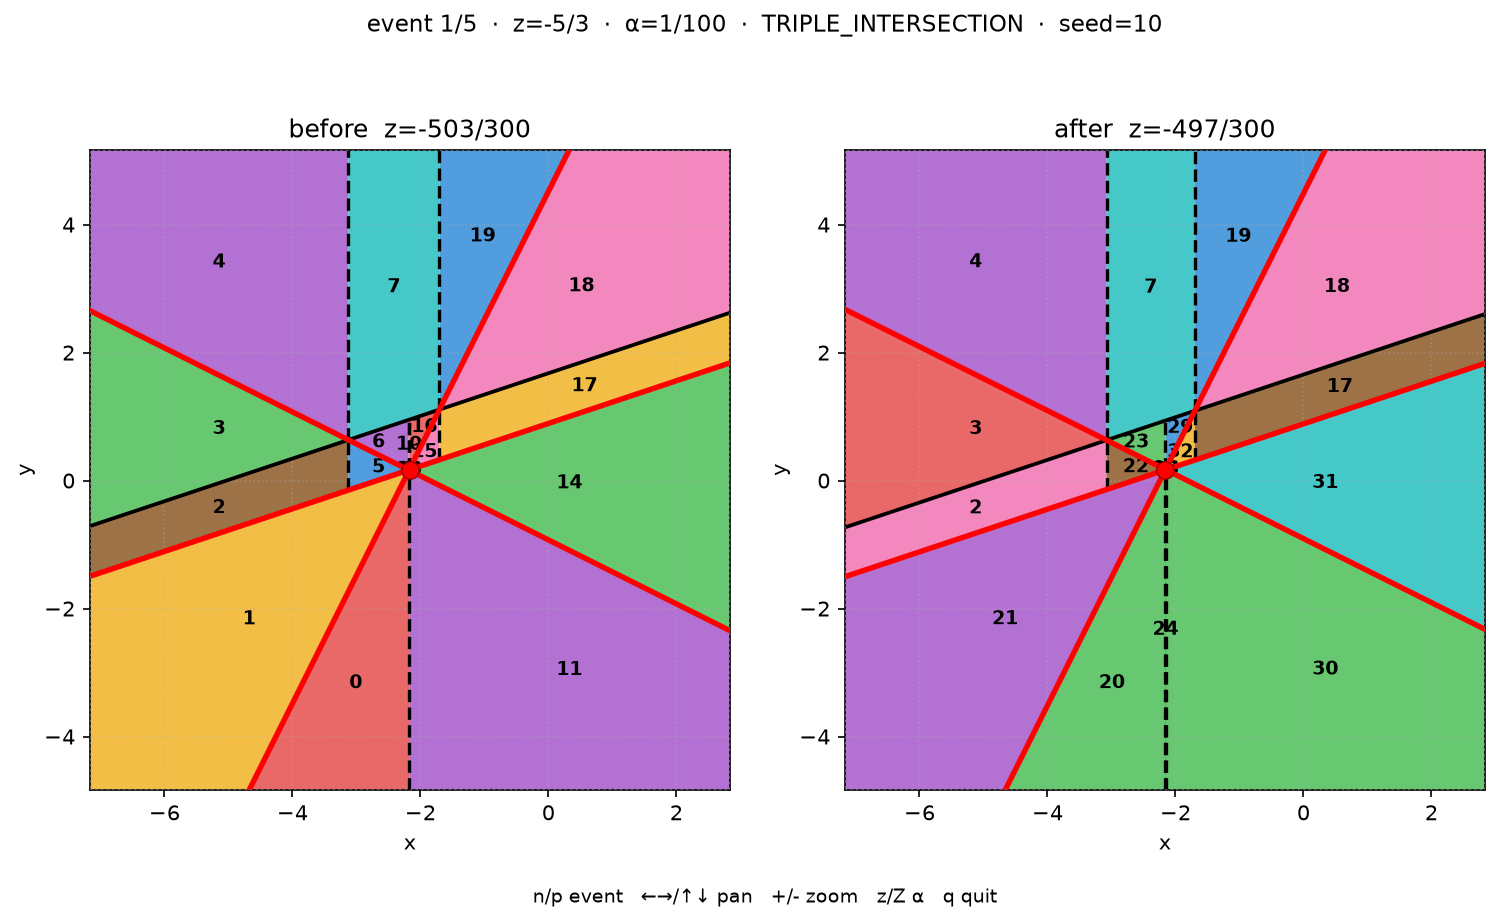
\includegraphics[width=\textwidth]{figures/show-sweep-random-4-seed-10.png}
\caption{\texttt{python -m vd3d --random-planes 4 --seed 10 --show-sweep}.
Sweep-plane vertical decomposition immediately before (left) and after (right)
the first event.  Solid: slice lines of the input planes.  Dashed: 2D-vertical
decomposition walls.  Colours: cell matching across the event.  Red: the event.}
\label{fig:showsweep}
\end{figure}

This instance is also a reminder of how easily random integer coefficients
violate general position.  The CLI reports

\begin{lstlisting}
warning: 2 events share z=-1/2 (TRIPLE_INTERSECTION, TRIPLE_INTERSECTION);
         planes are not in general position
planes: 4   events: 6   intervals: 6   cells: 70
\end{lstlisting}

With coefficients drawn from $\{-4,\dots,4\}$, coincidences at the same height
are common, which is why the event-group machinery is exercised constantly
rather than being an exotic corner.

\section{Benchmarks}
\label{sec:benchmarks}

\subsection{Setup}

All measurements were taken on a 13th Gen Intel Core i5-13420H (12 threads,
4.6\,GHz max) running Ubuntu 26.04 and CPython 3.14.4, single-threaded.
Instances are produced by \texttt{random\_general\_position\_planes}, which
draws integer coefficients uniformly from $\{-4,\dots,4\}$ and rejects a
candidate that is parallel to an existing plane, that makes some triple
singular, or that creates a $z$-parallel intersection line.  For each $n$ we
use seeds $1,\dots,20$ ($1,\dots,12$ for $n=8$) and run each instance twice:
once on the incremental path, once on the reference path.  Timings exclude
process startup and plane sampling.  Instances that abort
(Section~\ref{sec:robustness}) are excluded from timing statistics and counted
separately.

\subsection{Combinatorial growth}

Table~\ref{tab:combinatorics} reports the size of the instances.  The triple
count is exactly $\binom{n}{3}$, as it must be when every triple of sampled
planes is non-singular.  Alignment events are not merely present but dominant
from $n = 6$ upward: at $n = 8$ the median instance has 56 triples and 76
alignments, so the event type specific to vertical decomposition outnumbers the
event type shared with a plain arrangement sweep.

Fitting a power law $\log(\text{size})$ against $\log n$ over the measured
range gives
\[
  \text{slice trapezoids} \sim n^{2.0},\qquad
  \text{events} \sim n^{4.9},\qquad
  \text{3D cells} \sim n^{4.2}.
\]
The first of these is the theoretical bound: a slice is a trapezoidal map of
$n$ lines and has $\Theta(n^2)$ cells, and the fit recovers the exponent to two
digits.  The other two exceed their asymptotic bounds of $O(n^3)$, and this
should be read as a small-$n$ artefact rather than as a contradiction.  Over
$3 \le n \le 8$ the lower-order terms of the exact cell count are of the same
magnitude as the leading term --- for $n = 8$, $\binom{n}{3} = 56$ against
$\binom{n}{2} + \binom{n}{1} + 1 = 37$ --- so a log-log fit on this range
systematically overestimates the exponent.  The honest statement is that the
range is too narrow to measure asymptotics; what it does establish is that
alignment events are a first-order phenomenon, not a rare correction.

\begin{table}[htbp]
\centering
\begin{tabular}{rrrrrrrr}
\toprule
$n$ & inst. & triples & \multicolumn{2}{c}{alignments} & \multicolumn{2}{c}{3D cells} & slice cells \\
& & $\binom{n}{3}$ & med & max & med & max & med \\
\midrule
3 & 20 & 1 & 0 & 0 & 26 & 26 & 13 \\
4 & 20 & 4 & 2 & 3 & 84 & 89 & 23 \\
5 & 20 & 10 & 8 & 13 & 178 & 248 & 36 \\
6 & 20 & 20 & 23 & 28 & 435 & 481 & 52 \\
7 & 20 & 35 & 43 & 57 & 885 & 1018 & 71 \\
8 & 12 & 56 & 76 & 86 & 1633 & 1738 & 93 \\
\bottomrule
\end{tabular}
\caption{Instance sizes on random general-position planes (seeds $1..20$; $1..12$ for $n=8$). ``slice cells'' is the number of trapezoids in the initial slice decomposition. Cell statistics are over instances that completed.}
\label{tab:combinatorics}
\end{table}


\subsection{Running time}

Table~\ref{tab:timing} reports wall-clock time.  Two observations.

\begin{table}[htbp]
\centering
\begin{tabular}{rrrrrrrr}
\toprule
& \multicolumn{3}{c}{reference path (s)} & \multicolumn{3}{c}{incremental path (s)} & \\
\cmidrule(lr){2-4}\cmidrule(lr){5-7}
$n$ & median & max & per event & median & max & per event & ratio \\
\midrule
3 & 0.010 & 0.010 & 0.0097 & 0.012 & 0.013 & 0.0124 & 1.28 \\
4 & 0.105 & 0.165 & 0.0154 & 0.148 & 0.176 & 0.0216 & 1.40 \\
5 & 0.529 & 0.775 & 0.0279 & 0.798 & 1.092 & 0.0394 & 1.51 \\
6 & 2.286 & 3.335 & 0.0548 & 3.622 & 4.776 & 0.0785 & 1.58 \\
7 & 7.967 & 12.791 & 0.1077 & 14.619 & 19.779 & 0.1783 & 1.83 \\
8 & 28.239 & 32.618 & 0.2097 & 41.563 & 52.905 & 0.3012 & 1.47 \\
\midrule
\multicolumn{8}{l}{Power-law fit of median time: reference $t \propto n^{8.0}$, incremental $t \propto n^{8.3}$.} \\
\bottomrule
\end{tabular}
\caption{Wall-clock time, single-threaded. ``per event'' is median total time divided by the number of events. ``ratio'' is incremental median over reference median: values above $1$ mean the incremental path is slower, because it also recomputes the slice to assert agreement.}
\label{tab:timing}
\end{table}


First, the \textbf{growth rate is very steep}: a least-squares fit of $\log t$
against $\log n$ gives $t \propto n^{8.0}$ for the reference path and
$t \propto n^{8.3}$ for the incremental path.  Figure~\ref{fig:time-constructions}
plots both against the envelope construction.  This is not the complexity of
vertical decomposition; it is the complexity of this implementation, and it
decomposes cleanly.  Total time is (number of events) $\times$ (cost per
event), and the two factors are measured separately: the event count grows as
$n^{4.9}$ over this range, and the per-event cost --- last column pair of
Table~\ref{tab:timing} --- grows as $n^{3.1}$, from $9.7$\,ms at $n = 3$ to
$210$\,ms at $n = 8$.  Their product is the observed $n^{8}$.

The per-event $n^{3.1}$ is the actionable half.  Each event triggers two
from-scratch recomputations of the slice decomposition, and a single such
recomputation is itself superquadratic in $n$ even though its output has only
$\Theta(n^2)$ trapezoids.  The reason is a linear search in the planar layer:
assigning each trapezoid representative to its containing arrangement face
tests that point against \emph{every} face, which is $\Theta(n^2)$ faces at
$\Theta(n)$ cost each, for $\Theta(n^2)$ trapezoids.  Section~\ref{sec:future}
lists this as the first structural fix after the recomputation itself.

Second, the \textbf{incremental path is slower than the reference path}, by a
median factor of $1.3$ at $n = 3$ rising to $1.5$ at $n = 8$ when compared
instance by instance on the runs where both paths complete.  This is by
construction, not by accident: as described in Section~\ref{sec:verification}, the incremental path
computes the local update and \emph{also} recomputes $\VD^+$ to assert
agreement.  Making the incremental path faster than the reference path requires
dropping that assertion behind a flag, which the project has deliberately not
yet done.

\subsection{Cost breakdown}

Table~\ref{tab:breakdown} separates event generation from the sweep proper.
Triple generation is negligible.  Alignment generation is more expensive ---
it builds an $n$-line arrangement and a zone for each of the $\binom{n}{2}$
intersection lines --- but it remains a small fraction of total time, which is
dominated by the per-event slice work.  The single-slice column is the cost of
one from-scratch \texttt{compute\_vd\_at\_z}; multiplying it by twice the event
count accounts for most of the total.

\begin{table}[htbp]
\centering
\begin{tabular}{rrrrrr}
\toprule
$n$ & triples (s) & alignments (s) & one slice VD (s) & total sweep (s) & event gen.\ share \\
\midrule
3 & 0.00005 & 0.0009 & 0.0026 & 0.012 & 7.6\% \\
4 & 0.00018 & 0.0047 & 0.0062 & 0.138 & 3.7\% \\
5 & 0.00045 & 0.0165 & 0.0144 & 0.819 & 2.1\% \\
6 & 0.00086 & 0.0473 & 0.0306 & 3.348 & 1.4\% \\
7 & 0.00150 & 0.1130 & 0.0571 & 11.951 & 1.0\% \\
\bottomrule
\end{tabular}
\caption{Cost breakdown (medians, 8 seeds per $n$, reference path). ``one slice VD'' is a single from-scratch \texttt{compute\_vd\_at\_z}. The last column is event generation as a fraction of total sweep time.}
\label{tab:breakdown}
\end{table}


\subsection{The hypograph construction}
\label{sec:bench-hypograph}

Table~\ref{tab:hypograph} runs the hypograph pipeline on the same instances.
The contrast with Table~\ref{tab:timing} is stark in three ways.

\begin{table}[htbp]
\centering
\begin{tabular}{rrrrrrrrr}
\toprule
& & & envelope & \multicolumn{2}{c}{hypograph cells} & hypograph & full sweep & \\
\cmidrule(lr){5-6}
$n$ & inst. & active & facets & med & max & time (s) & time (s) & speed-up \\
\midrule
3 & 20 & 3 & 1 & 5 & 5 & 0.0009 & 0.02 & ${\sim}24\times$ \\
4 & 20 & 4 & 2 & 8 & 10 & 0.0022 & 0.27 & ${\sim}119\times$ \\
5 & 20 & 5 & 3 & 11 & 15 & 0.0034 & 1.47 & ${\sim}435\times$ \\
6 & 20 & 5 & 4 & 13 & 21 & 0.0054 & 6.43 & ${\sim}847\times$ \\
7 & 20 & 5 & 4 & 14 & 26 & 0.0059 & 21.80 & ${\sim}3305\times$ \\
\midrule
\multicolumn{9}{l}{Completed: hypograph 100/100; full sweep 64/100. Float/exact disagreements: 0.} \\
\bottomrule
\end{tabular}
\caption{The hypograph construction on the same random instances as Table~\ref{tab:timing} (seeds $1..20$). ``active'' is the number of planes that appear on the lower envelope; ``facets'' the number of envelope vertices (dual lower-hull triangles). ``hypograph time'' is exact envelope plus exact hypograph VD; ``full sweep time'' and the speed-up are medians over the instances where the sweep also completed.}
\label{tab:hypograph}
\end{table}


\emph{Size.} Cells grow as $n^{1.24}$ and envelope facets as $n^{1.70}$ over
this range, against $n^{4.2}$ for the sweep's cell count.  The medians already
flatten --- the number of \emph{active} planes stalls at 5 from $n = 5$ onward,
because a plane drawn at random is increasingly likely not to reach the lower
envelope at all.  This range is far too short to fit an exponent to, and
Section~\ref{sec:bench-env-scaling} shows that both of these numbers are
artefacts of it; they are quoted here only to make the contrast with the sweep
on identical instances.

\emph{Speed.} Exact envelope plus exact hypograph VD takes $6$\,ms at $n = 7$,
where the full sweep takes $22$\,s (Figure~\ref{fig:time-constructions}): a
median speed-up of ${\sim}3\,300\times$,
rising monotonically with $n$ because the two have different exponents
($n^{2.29}$ against $n^{8.0}$).  The $O(n^4)$ brute-force hull enumeration is
not the bottleneck at these sizes: the exact envelope takes a median
$0.10$\,ms at $n = 3$ rising to $1.17$\,ms at $n = 7$ (largest observed
$1.73$\,ms), so the trapezoid construction, not the hull, dominates the
millisecond budget.

\emph{Robustness.} All 100 instances completed, with zero float-versus-exact
disagreements.  The full sweep completed on 64 of the same 100.  Of the 36
instances where the sweep aborted and the hypograph pipeline did not, 24 were
class (a) and 12 class (b) of Section~\ref{sec:robustness} --- which is what one
would expect, since the hypograph package touches neither the
\texttt{arrangement2d} DCEL whose face extraction carries defect (a) nor the
event machinery that carries (b).  It is not that this construction is more
carefully written; it is that it is a much shorter path through much less code
--- 1\,558 lines of kernel against 5\,613 for the sweep.

\subsection{Scaling beyond the sweep's range}
\label{sec:bench-env-scaling}

Section~\ref{sec:bench-hypograph} ran the envelope path only where the sweep
could be run too, which wastes most of its range.  Table~\ref{tab:env-random}
takes it to $n = 96$.  Two changes of instance distribution are needed and
should be stated plainly: the library's own
\texttt{random\_general\_position\_planes} draws coefficients from
$\{-4,\dots,4\}$ and \emph{cannot} deliver more than about 25 planes in general
position --- it raises \texttt{RuntimeError} at $n = 26$, having exhausted the
$9^4$ available coefficient tuples --- so these runs use a local sampler with
coefficients in $\{-50,\dots,50\}$.  And since the envelope construction needs
only $c \neq 0$, not full general position, the sampler does not enforce one.

The headline is that on random input this construction barely grows at all:
\[
  \text{active planes} \sim n^{0.14}, \qquad
  \text{envelope facets} \sim n^{0.31}, \qquad
  \text{cells} \sim n^{0.26}.
\]
Six or seven planes reach the envelope whether $n$ is 8 or 96, and the output is
some 25 cells throughout.  This is not the $\Theta(n)$ of
Proposition~\ref{prop:envelope-linear}; it is the well-known fact that the
convex hull of $n$ uniformly random points in a convex body has expected
complexity polylogarithmic in $n$, and the lower hull of the dual points
inherits it.  The $n^{1.24}$ cell growth reported in
Section~\ref{sec:bench-hypograph} was an artefact of fitting over $3 \le n \le
7$, where almost every plane is still active; it should not have been called
consistent with the linear bound, and the wider range corrects it.

\begin{figure}[htbp]
\centering
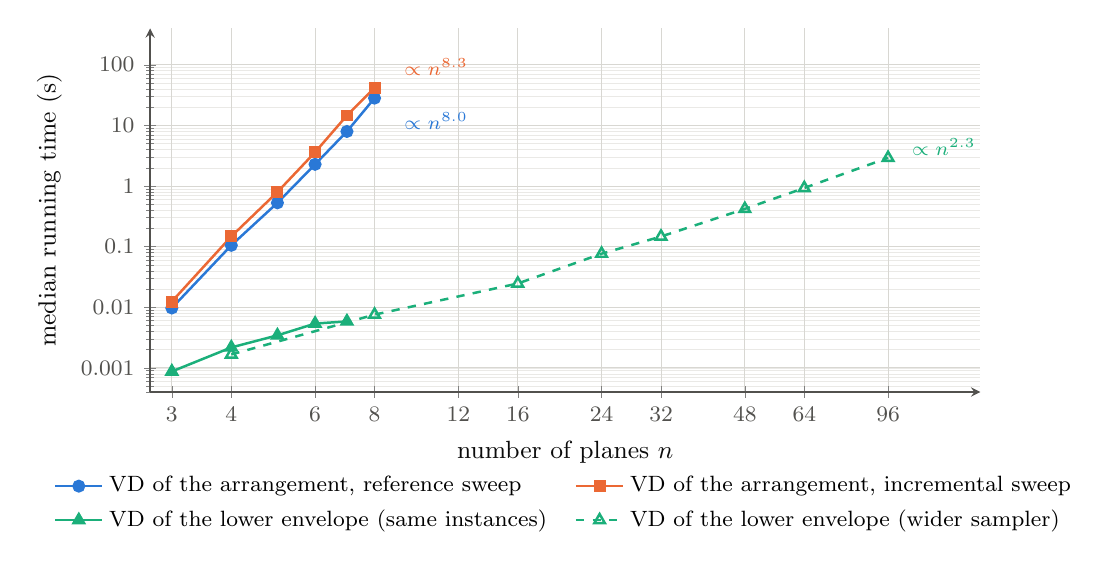
\begin{tikzpicture}
\begin{axis}[
    width=\linewidth, height=6.2cm,
    xmode=log, ymode=log, log basis x=10,
    xlabel={number of planes $n$}, ylabel={median running time (s)},
    xtick={3,4,6,8,12,16,24,32,48,64,96}, xticklabels={3,4,6,8,12,16,24,32,48,64,96},
    ytick={1e-4,1e-3,1e-2,1e-1,1,1e1,1e2},
    log ticks with fixed point,
    xmin=2.7, xmax=150,
    ymin=4e-4, ymax=4e2,
    grid=both,
    major grid style={line width=0.3pt, draw=gridgray},
    minor grid style={line width=0.2pt, draw=gridgray, opacity=0.55},
    axis lines=left, axis line style={draw=inktwo, line width=0.5pt},
    tick label style={font=\footnotesize, color=inktwo},
    label style={font=\small, color=ink},
    legend cell align=left,
    legend style={draw=none, fill=none, font=\footnotesize,
                  at={{(0.5,-0.20)}}, anchor=north, row sep=1pt,
                  /tikz/every even column/.append style={column sep=8pt}},
    legend columns=2,
]
\addplot[serA, line width=0.9pt, mark=*, mark size=1.9pt]
  coordinates {(3,0.00974126) (4,0.105319) (5,0.529164) (6,2.28555) (7,7.967) (8,28.2387)};
\addlegendentry{VD of the arrangement, reference sweep}
\addplot[serB, line width=0.9pt, mark=square*, mark size=1.7pt]
  coordinates {(3,0.0124374) (4,0.147618) (5,0.797553) (6,3.62193) (7,14.6194) (8,41.5625)};
\addlegendentry{VD of the arrangement, incremental sweep}
\addplot[serC, line width=0.9pt, mark=triangle*, mark size=2.2pt]
  coordinates {(3,0.0008735) (4,0.00217614) (5,0.00344401) (6,0.0053871) (7,0.00585255)};
\addlegendentry{VD of the lower envelope (same instances)}
\addplot[serC, line width=0.9pt, dashed, mark=triangle, mark size=2.2pt,
         mark options={solid, fill=white}]
  coordinates {(4,0.00166616) (8,0.00756478) (16,0.0246835) (24,0.0766006) (32,0.147123) (48,0.419906) (64,0.929787) (96,2.92514)};
\addlegendentry{VD of the lower envelope (wider sampler)}
\node[serB, font=\scriptsize, anchor=west] at (axis cs:8.8,91.44)
  {$\propto n^{8.3}$};
\node[serA, font=\scriptsize, anchor=west] at (axis cs:8.8,11.86)
  {$\propto n^{8.0}$};
\node[serC, font=\scriptsize, anchor=west] at (axis cs:102.72,4.388)
  {$\propto n^{2.3}$};
\end{axis}
\end{tikzpicture}
\caption{Median running time of the two constructions, log--log.  Both sweep
paths and the solid envelope series are the general-position instances of
Tables~\ref{tab:timing} and \ref{tab:hypograph} (coefficients in
$\{-4,\dots,4\}$, $n \le 8$); the dashed envelope series is the wider sampler of
Table~\ref{tab:env-random}, which reaches $n = 96$.  The two distributions agree
where they overlap.  Exponents are least-squares fits over each series' own
range; the sweep's is measured over $3 \le n \le 8$ and is not an asymptotic
claim (Section~\ref{sec:bench-env-scaling}).}
\label{fig:time-constructions}
\end{figure}


Running time, by contrast, grows steeply: $t_{\text{hull}} \sim n^{2.99}$,
which is the $O(n^4)$ triple enumeration of \texttt{lower\_hull\_facets}
paying off only partially from early rejection.  By $n = 96$ the hull
enumeration takes $2.4$\,s and dominates the trapezoid construction's
$0.47$\,s, inverting the ordering seen at $n \le 7$; Figure~\ref{fig:time-stages}(a)
puts the crossover at $n \approx 26$.  So the construction is
cheap for the reason that its \emph{output} is small on random input, not
because its inner loops are efficient.

\begin{table}[htbp]
\centering
\begin{tabular}{rrrrrrrr}
\toprule
$n$ & active & env.\ facets & cells & $t_{\text{hull}}$ (s) & $t_{\text{trap}}$ (s) & float (s) & exact/float \\
\midrule
4 & 4 & 2 & 10 & 0.0002 & 0.0015 & 0.0007 & $2.3\times$ \\
8 & 6 & 5 & 24 & 0.0012 & 0.0064 & 0.0022 & $3.5\times$ \\
16 & 6 & 6 & 23 & 0.0103 & 0.0150 & 0.0051 & $5.2\times$ \\
24 & 7 & 7 & 34 & 0.0354 & 0.0410 & 0.0123 & $6.3\times$ \\
32 & 7 & 6 & 26 & 0.0877 & 0.0594 & 0.0182 & $8.7\times$ \\
48 & 7 & 6 & 26 & 0.3057 & 0.1199 & 0.0419 & $9.6\times$ \\
64 & 7 & 7 & 28 & 0.7248 & 0.2312 & 0.0798 & $12.1\times$ \\
96 & 6 & 6 & 29 & 2.4191 & 0.4739 & 0.1673 & $17.6\times$ \\
\midrule
\multicolumn{8}{l}{Fits: active ${\sim}n^{0.14}$, facets ${\sim}n^{0.31}$, cells ${\sim}n^{0.26}$, $t_{\text{hull}} {\sim} n^{2.99}$, $t_{\text{trap}} {\sim} n^{1.79}$. Float/exact agreement: 80/80.} \\
\bottomrule
\end{tabular}
\caption{Hypograph construction on random planes, coefficients drawn uniformly from $\{-50,\dots,50\}$ with $c \neq 0$, medians over 10 seeds. $t_{\text{hull}}$ is the exact lower-hull envelope, $t_{\text{trap}}$ the exact trapezoid construction; ``float'' is both stages via Qhull. ``active'' is the number of planes appearing on the envelope.}
\label{tab:env-random}
\end{table}


\subsection{A family where $\Theta(n)$ is attained}
\label{sec:bench-voronoi}

To exercise the bound rather than the average case we need instances whose dual
points all reach the lower hull.  The classical lifting supplies them: map a
site $s_i = (a_i, b_i)$ to
\[
  P_i:\quad 2 a_i x + 2 b_i y + z - (a_i^2 + b_i^2) = 0,
  \qquad\text{so}\qquad
  f_i(x,y) = \lVert (x,y) - s_i \rVert^2 - (x^2 + y^2).
\]
The subtracted term is common to all planes, so the minimization diagram of
$\{f_i\}$ is exactly the \textbf{Voronoi diagram} of the sites, and the dual
points $(2a_i, 2b_i, a_i^2{+}b_i^2)$ lie on a paraboloid, hence all on the lower
hull.  Table~\ref{tab:env-voronoi} confirms both: every one of the $n$ planes is
active at every size tested, and the facet count converges to
$\approx 1.8n$, consistent with the $2n - 2 - h$ triangles of a Delaunay
triangulation.

This family also provides a semantic oracle that costs nothing to state: the
ceiling plane of the cell containing a point must be the plane of that point's
\emph{nearest site}.  Over 10\,500 sample points at exact rational coordinates
across all sizes and seeds, there were no violations.  That checks the whole
pipeline --- duality, hull, minimization diagram, trapezoids and the lift ---
against an independently computed nearest-neighbour, and it is a stronger
statement than the float/exact cross-check, which only says the two
implementations agree with each other.

\begin{table}[htbp]
\centering
\begin{tabular}{rrrrrrrr}
\toprule
$n$ & active & env.\ facets & facets$/n$ & cells & cells$/n$ & $t_{\text{hull}}$ (s) & $t_{\text{trap}}$ (s) \\
\midrule
4 & 4 & 2 & 0.50 & 10 & 2.5 & 0.000 & 0.001 \\
8 & 8 & 9 & 1.12 & 44 & 5.5 & 0.001 & 0.010 \\
16 & 16 & 23 & 1.44 & 170 & 10.6 & 0.010 & 0.087 \\
24 & 24 & 38 & 1.58 & 334 & 13.9 & 0.037 & 0.285 \\
32 & 32 & 53 & 1.66 & 502 & 15.7 & 0.087 & 0.650 \\
48 & 48 & 85 & 1.77 & 961 & 20.0 & 0.316 & 2.090 \\
64 & 64 & 115 & 1.80 & 1423 & 22.2 & 0.777 & 4.927 \\
\midrule
\multicolumn{8}{l}{All $n$ planes active in every instance. Fits: facets ${\sim}n^{1.42}$, cells ${\sim}n^{1.78}$. Nearest-site check: 0/10500 wrong.} \\
\bottomrule
\end{tabular}
\caption{The Voronoi lifting: site $(a,b) \mapsto 2ax + 2by + z - (a^2{+}b^2) = 0$, sites drawn from $\{-200,\dots,200\}^2$, medians over 5 seeds. Every plane reaches the envelope, and the minimization diagram is the Voronoi diagram of the sites, so the envelope has $\Theta(n)$ complexity. The nearest-site check verifies that the ceiling of the cell containing a sample point is the plane of its nearest site.}
\label{tab:env-voronoi}
\end{table}


\begin{figure}[htbp]
\centering
\begin{minipage}{0.49\textwidth}\centering
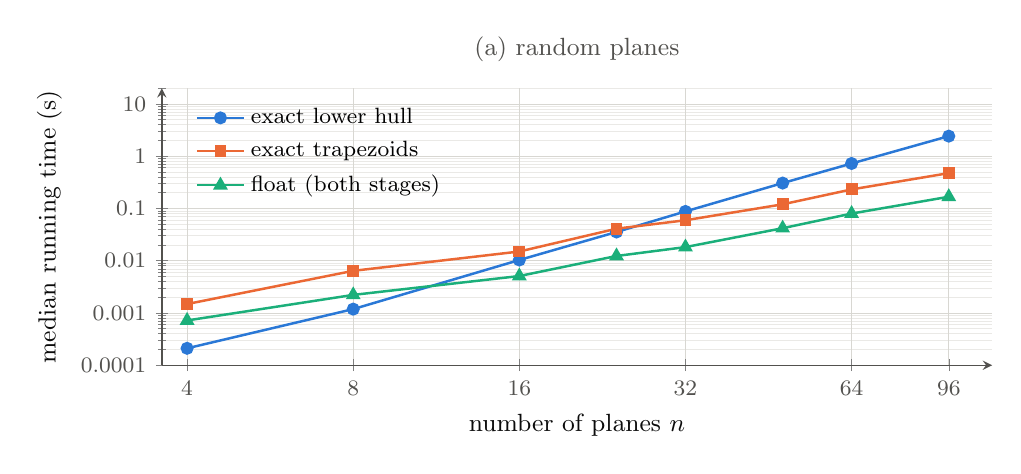
\begin{tikzpicture}
\begin{axis}[
    width=\linewidth, height=5.1cm,
    xmode=log, ymode=log, log basis x=10,
    xlabel={number of planes $n$}, ylabel={median running time (s)},
    xtick={4,8,16,32,64,96}, xticklabels={4,8,16,32,64,96},
    ytick={1e-4,1e-3,1e-2,1e-1,1,1e1,1e2},
    log ticks with fixed point,
    xmin=3.6, xmax=115,
    ymin=1e-4, ymax=2e1,
    grid=both,
    major grid style={line width=0.3pt, draw=gridgray},
    minor grid style={line width=0.2pt, draw=gridgray, opacity=0.55},
    axis lines=left, axis line style={draw=inktwo, line width=0.5pt},
    tick label style={font=\footnotesize, color=inktwo},
    label style={font=\small, color=ink},
    legend cell align=left,
    legend style={draw=none, fill=none, font=\footnotesize,
                  at={{(0.03,0.97)}}, anchor=north west, row sep=1pt,
                  /tikz/every even column/.append style={column sep=8pt}},
    legend columns=1,
    title={(a) random planes}, title style={font=\small, color=inktwo},
]
\addplot[serA, line width=0.9pt, mark=*, mark size=1.9pt] coordinates {(4,0.000210729) (8,0.00118501) (16,0.010316) (24,0.035423) (32,0.0877028) (48,0.30565) (64,0.724792) (96,2.41906)};
\addlegendentry{exact lower hull}
\addplot[serB, line width=0.9pt, mark=square*, mark size=1.7pt] coordinates {(4,0.00148226) (8,0.00639972) (16,0.0149908) (24,0.0409703) (32,0.0594197) (48,0.119924) (64,0.231151) (96,0.473851)};
\addlegendentry{exact trapezoids}
\addplot[serC, line width=0.9pt, mark=triangle*, mark size=2.2pt] coordinates {(4,0.000718652) (8,0.00221655) (16,0.00508758) (24,0.0123112) (32,0.0182174) (48,0.0418716) (64,0.0798031) (96,0.167312)};
\addlegendentry{float (both stages)}
\end{axis}
\end{tikzpicture}
\end{minipage}\hfill
\begin{minipage}{0.49\textwidth}\centering
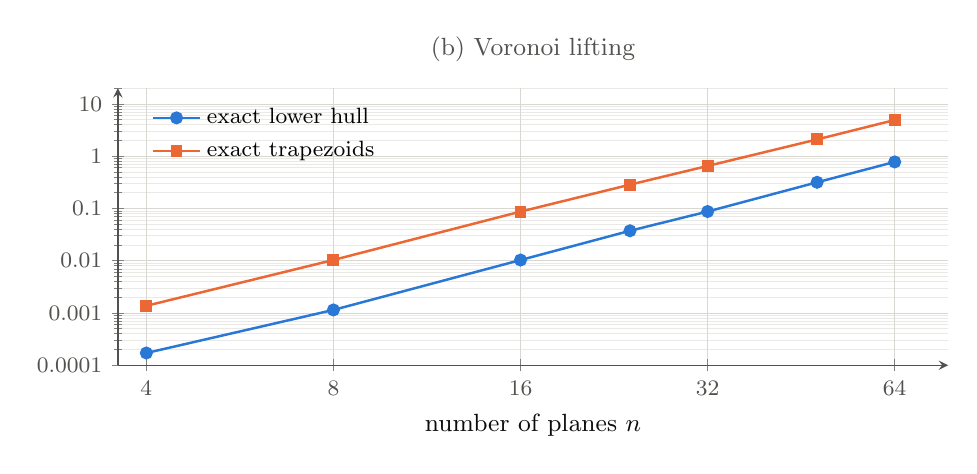
\begin{tikzpicture}
\begin{axis}[
    width=\linewidth, height=5.1cm,
    xmode=log, ymode=log, log basis x=10,
    xlabel={number of planes $n$}, ylabel={},
    xtick={4,8,16,32,64}, xticklabels={4,8,16,32,64},
    ytick={1e-4,1e-3,1e-2,1e-1,1,1e1,1e2},
    log ticks with fixed point,
    xmin=3.6, xmax=78,
    ymin=1e-4, ymax=2e1,
    grid=both,
    major grid style={line width=0.3pt, draw=gridgray},
    minor grid style={line width=0.2pt, draw=gridgray, opacity=0.55},
    axis lines=left, axis line style={draw=inktwo, line width=0.5pt},
    tick label style={font=\footnotesize, color=inktwo},
    label style={font=\small, color=ink},
    legend cell align=left,
    legend style={draw=none, fill=none, font=\footnotesize,
                  at={{(0.03,0.97)}}, anchor=north west, row sep=1pt,
                  /tikz/every even column/.append style={column sep=8pt}},
    legend columns=1,
    title={(b) Voronoi lifting}, title style={font=\small, color=inktwo},
]
\addplot[serA, line width=0.9pt, mark=*, mark size=1.9pt] coordinates {(4,0.000171292) (8,0.00114329) (16,0.0103008) (24,0.0373715) (32,0.0872819) (48,0.316407) (64,0.776608)};
\addlegendentry{exact lower hull}
\addplot[serB, line width=0.9pt, mark=square*, mark size=1.7pt] coordinates {(4,0.00137033) (8,0.0103296) (16,0.0869927) (24,0.285026) (32,0.650248) (48,2.09001) (64,4.92729)};
\addlegendentry{exact trapezoids}
\end{axis}
\end{tikzpicture}
\end{minipage}
\caption{The envelope pipeline's two exact stages, log--log.  \textbf{(a)} On
random planes the $O(n^4)$ hull enumeration overtakes the trapezoid
construction at $n \approx 26$ and is $5.1\times$ its cost by
$n = 96$, because the envelope --- and therefore the trapezoid work --- stops
growing while the triple enumeration does not.  \textbf{(b)} On the Voronoi
lifting the ordering is reversed at every size: all $n$ planes stay active, so
the trapezoid stage has $\Theta(n)$ envelope features to decompose and dominates
throughout.  Panel (a) also shows the price of exactness, as the gap between the
two exact stages and the float series.}
\label{fig:time-stages}
\end{figure}


\subsection{The merge step never fires}
\label{sec:bench-merge}

The Voronoi family also exposes a defect.  Cells grow as $n^{1.78}$ here, not
$\Theta(n)$: at $n = 64$ the diagram has 113 vertices, whose trapezoidal map
should have a few hundred cells, and the implementation emits 1\,423.  The
ratio of emitted cells to $3 \times (\text{envelope vertices})$ climbs
steadily --- $1.7, 2.8, 3.3, 3.8, 4.2$ for $n = 8 \dots 64$ --- so the
over-refinement is not a constant factor.

Instrumenting \texttt{build\_trapezoids} locates it exactly.  The routine first
cuts the plane into vertical strips at every envelope-vertex abscissa and lists
the $y$-bands inside each strip, then runs a merge loop intended to rejoin
adjacent strip pieces that belong to the same envelope face and the same band.
Counting pieces before and after that loop:

\begin{center}
\begin{tabular}{rrrr}
\toprule
$n$ (Voronoi) & pieces before merge & cells after & merged away \\
\midrule
8  & 56    & 56    & 0 \\
16 & 199   & 199   & 0 \\
32 & 517   & 517   & 0 \\
48 & 965   & 965   & 0 \\
64 & 1\,423 & 1\,423 & 0 \\
\bottomrule
\end{tabular}
\end{center}

Not one merge, at any size.  The same holds on the random family and on
\texttt{examples/three\_planes.txt}.  The cause is the merge predicate: it
accepts two adjacent pieces only when their recorded band bounds are
\emph{numerically equal}, but those bounds are the $y$-values of the bounding
diagram edges sampled at each strip's own midpoint.  For a band bounded by an
edge of non-zero slope those two numbers necessarily differ, so the test fails.
At $n = 32$ there are 485 adjacent piece pairs that share an envelope face ---
every one a legitimate merge candidate --- and zero of them pass.  The merge
needs to compare the \emph{combinatorial identity} of the bounding edges, not
sampled ordinates.

The consequence is that the package computes a vertical \emph{slab}
decomposition --- one cell per strip per band --- rather than a trapezoidal map.
It is still a valid decomposition into constant-complexity prisms, and the
partition oracle of Section~\ref{sec:bench-oracle} passes on it, so nothing
downstream is wrong; it is simply larger than it needs to be, by a factor that
grows with $n$.  Proposition~\ref{prop:envelope-linear} bounds the trapezoidal
map, and should be read as a statement about the problem rather than about this
implementation.

\subsection{Exact arithmetic against Qhull}
\label{sec:bench-arith}

Having two implementations that differ only in arithmetic invites the obvious
experiment: widen the coefficient range and see when double precision breaks.
Table~\ref{tab:env-arith} does this over five decades.

The result runs opposite to expectation.  Disagreements appear only at the
\emph{narrowest} range, coefficients in $\{-4,\dots,4\}$: 3 instances out of 30,
against 0 out of 30 at every wider range including $10^{12}$.  Qhull's vertex
coordinates stay accurate to $1.4 \times 10^{-13}$ throughout.  Small integer
coefficients are not easy inputs, they are degenerate ones --- in the single
instance whose \emph{active set} differed, 344 of the $\binom{32}{4}$ subsets of
dual points are exactly coplanar.

\begin{remark}[the exact path over-reports under degeneracy]
\label{rem:degenerate-facets}
In that instance the exact path reports 8 active planes and 11 facets, Qhull 7
and 8.  The extra plane is the strict minimum nowhere: on an $81 \times 81$
exact rational grid it attains the minimum at exactly one point and ties there.
Its dual point lies \emph{on} the plane of a lower-hull facet without being a
vertex of the hull, and \texttt{is\_lower\_hull\_facet} admits it, because the
rejection test is $(q - p_i) \cdot n > 0$ --- points exactly on the supporting
plane pass.  Every triple of coplanar points on one hull face therefore counts
as its own facet.  Qhull merges coplanar facets and reports the minimal set.

So the disagreement is about the representation of a degenerate face, not about
a sign computed wrongly, and the exactly-computed answer is the less useful of
the two.  Note where it does \emph{not} propagate: the hypograph VD agreed in
all three cases (column 6 of Table~\ref{tab:env-arith}), because a plane that
contributes no two-dimensional face contributes no cell.  Exactness guarantees
the true sign of each predicate; it does not supply a canonical answer when the
object being computed is not unique.
\end{remark}

Exactness is not free, and it gets dearer in two independent directions.  Across
Table~\ref{tab:env-arith} the exact pipeline costs $4.0\times$ the float one at
coefficient bound 4 and $12.4\times$ at $10^{12}$, at fixed $n$; across
Table~\ref{tab:env-random} it rises from $2.3\times$ at $n = 4$ to $17.6\times$
at $n = 96$, at fixed coefficient bound.  Both trends are the same mechanism:
the rationals carried through the pipeline get longer.

\begin{table}[htbp]
\centering
\begin{tabular}{rrrrrrr}
\toprule
coeff.\ bound & inst. & disagree & active set & facet set & hypograph VD & exact/float \\
\midrule
$4$ & 30 & 3 & 1 & 3 & 0 & $4.0\times$ \\
$50$ & 30 & 0 & 0 & 0 & 0 & $5.2\times$ \\
$1\,000$ & 30 & 0 & 0 & 0 & 0 & $6.2\times$ \\
$1\,000\,000$ & 30 & 0 & 0 & 0 & 0 & $8.8\times$ \\
$1\,000\,000\,000\,000$ & 30 & 0 & 0 & 0 & 0 & $12.4\times$ \\
\bottomrule
\end{tabular}
\caption{Exact arithmetic against Qhull as the coefficient range widens; $n \in \{8,16,32\}$, 10 seeds each, so 30 instances per row. Columns 4--6 count the instances whose active plane set, lower-hull facet set, or final hypograph VD differed. Disagreements occur only at the \emph{narrowest} coefficient range, where degeneracies are common; see Remark~\ref{rem:degenerate-facets}.}
\label{tab:env-arith}
\end{table}


\subsection{Partition oracle at scale}
\label{sec:bench-oracle}

Section~\ref{sec:hypograph} reported the partition oracle on small instances.
Extending it to the wider sampler and to $n = 32$:

\begin{center}
\begin{tabular}{rrrrrrr}
\toprule
$n$ & cells & pts below & pts above & on boundary & gaps & overlaps \\
\midrule
4  & 12 & 2\,574 & 4\,925 & 1 & 0 & 0 \\
8  & 23 & 1\,548 & 5\,951 & 1 & 0 & 0 \\
16 & 18 & 1\,134 & 6\,366 & 0 & 0 & 0 \\
32 & 15 &   278  & 7\,222 & 0 & 0 & 0 \\
\bottomrule
\end{tabular}
\end{center}

30\,000 exact rational sample points over 20 instances, with no gaps, no
overlaps and no point above the envelope landing in a cell.  The fraction of
samples that fall below the envelope drops sharply with $n$ --- from $34\%$ to
$4\%$ --- because the envelope of more planes sits lower, which is worth noting
as a limitation of uniform sampling rather than a result: at larger $n$ most of
the budget is spent confirming the easy direction.

\subsection{Discussion}

The measurements support a clear statement of where the implementation
currently stands: it is a \emph{reference} implementation whose asymptotic
behaviour is dominated by the verification scaffolding and by naive inner loops
in the planar layer, not by anything intrinsic to the vertical decomposition.
The instance sizes it handles comfortably --- up to eight planes, a few
thousand cells, tens of seconds --- are adequate for developing and validating
the algorithm and for the visual review workflow, and inadequate for
application to real data.  The gap is not small, but it is also not mysterious;
Section~\ref{sec:future} lists the specific changes.

\section{Robustness evaluation}
\label{sec:robustness}

Reporting benchmarks without reporting failures would misrepresent the state of
the implementation.  Everything in this section concerns the \emph{sweep}; the
hypograph construction of Section~\ref{sec:hypograph} completed on every
instance we ran it on and is discussed at the end.

Of the 112 random instances used above ($n \in \{3,\dots,8\}$), the reference
path completes on $80$ ($71\%$) and the incremental path on $67$ ($60\%$); the
rest abort with an exception rather than returning a wrong answer.
Table~\ref{tab:failures} breaks this down.

\subsection{Failure taxonomy}

\begin{table}[htbp]
\centering
\begin{tabular}{rrrrrrr}
\toprule
& & \multicolumn{2}{c}{incremental path} & \multicolumn{2}{c}{reference path} & \\
\cmidrule(lr){3-4}\cmidrule(lr){5-6}
$n$ & inst. & class (a) & class (b) & class (a) & class (b) & completion rate \\
\midrule
3 & 20 & 1 & 0 & 1 & 0 & 95\% / 95\% \\
4 & 20 & 4 & 1 & 4 & 0 & 75\% / 80\% \\
5 & 20 & 5 & 2 & 5 & 0 & 65\% / 75\% \\
6 & 20 & 6 & 3 & 6 & 0 & 55\% / 70\% \\
7 & 20 & 8 & 6 & 9 & 0 & 30\% / 55\% \\
8 & 12 & 6 & 3 & 7 & 0 & 25\% / 42\% \\
\midrule
all & 112 & 30 & 15 & 32 & 0 & 60\% / 71\% \\
\bottomrule
\end{tabular}
\caption{Aborted runs by class. (a) face-extraction failure in the planar layer; (b) incremental-vs-reference divergence caught by the differential assertion. Completion rate is given as incremental / reference.}
\label{tab:failures}
\end{table}


Two classes appear.

\paragraph{(a) Face-extraction failure.}
The error surfaces downstream as
\begin{lstlisting}
error: representative Point2D(x=Fraction(-509, 600), y=Fraction(-3209, 1800))
       lies in 0 arrangement faces
\end{lstlisting}
raised when a trapezoid's interior representative point cannot be assigned to
any face of the slice arrangement.  This class occurs at essentially the same
rate on both paths (Table~\ref{tab:failures}; the differences of one are
instances where the incremental run aborts on class (b) at an earlier height),
which localises it to the planar layer rather than to the sweep.

\paragraph{(b) Incremental/reference divergence.}
The error is
\begin{lstlisting}
AssertionError: incremental 2D VD is not combinatorially equal to
                compute_vd_at_z(z+) for group z=-3 ids=['triple:1:2:3', ...]
\end{lstlisting}
which is the Layer-3 differential assertion firing.  It occurs only on the
incremental path, and in all 15 observed cases at an event \emph{group}: two or
more events sharing a height --- in every case a group of simultaneous triples,
with no alignment involved.  The reference path completes on those same
instances.
This is the verification architecture doing exactly its job --- the incremental
local update is not yet correct for all simultaneous-event configurations, and
the assertion refuses to let a wrong answer escape.

\subsection{Root cause of class (a)}

Class (a) is a genuine defect with a single root cause, which we located and
verified.  The smallest instance in our scans that reproduces it is
\verb|--random-planes 3 --seed 1|:
\[
  P_1: 3x + 3y + 3z + 2 = 0,\quad
  P_2: -x - 3y + 3z - 4 = 0,\quad
  P_3: 2x + 2y - 4z + 3 = 0 .
\]
Note that $P_1$ and $P_3$ have proportional $(a,b)$ but are not parallel
planes: their intersection line is \emph{horizontal} ($d_z = 0$), so their slice
lines are parallel at every height and coincide at exactly one height,
$z = 5/18$.  The sampler's general-position filter rejects $z$-parallel
intersection lines but not horizontal ones, so this configuration is admitted.

At $z = 241/900$, just below the coincidence height, the slice arrangement of
these three lines is built with
\[
  V = 2,\quad E = 7,\quad F = 2,
\]
so $V - E + F = -3$ rather than the required $1$: five faces are missing.  The
two faces that survive are two spuriously merged cycles.  The defect is in the
routine that links half-edges departing to infinity.  Rays are sorted by
direction and, for parallel rays, by their offset along the left normal of that
direction.  But the offset is computed from the \emph{unnormalised} direction
vector: the two parallel slice lines here have direction vectors $(3,-3)$ and
$(2,-2)$, so their left normals are $(3,3)$ and $(2,2)$ and the two offsets are
computed on different scales.  At $z = -13/18$ the comparison happens to give
the right order ($1/6$ versus $-53/9$); at $z = 241/900$ it gives the wrong one
($-841/300$ versus $-434/225$, while the true perpendicular offsets are
$-841/900$ and $-868/900$).  A single transposition in the cyclic order at
infinity merges the face cycles, the Euler check fails, and the trapezoid
representative lands in no face.

We verified the diagnosis by normalising the direction vector before taking the
left normal, i.e.\ dividing $(d_x,d_y)$ by $\max(|d_x|,|d_y|)$ in
\verb|_left_offset|, and re-running the robustness scan.  The result is
unambiguous:

\begin{center}
\begin{tabular}{lrrrr}
\toprule
scan: 160 instances, & \multicolumn{2}{c}{reference path} & \multicolumn{2}{c}{incremental path} \\
\cmidrule(lr){2-3}\cmidrule(lr){4-5}
$n \in \{3,\dots,6\}$, seeds $1..40$ & as shipped & normalised & as shipped & normalised \\
\midrule
completed          & 122 & \textbf{160} & 112 & 133 \\
class (a) aborts   & 38  & \textbf{0}   & 38  & \textbf{0} \\
class (b) aborts   & 0   & 0            & 10  & 27 \\
\bottomrule
\end{tabular}
\end{center}

With the fix the reference sweep completes on \emph{all} 160 instances of the
scan, and class (a) disappears entirely on both paths.  The incremental class
(b) count rises from 10 to 27, which is not a regression: those are instances
that previously aborted in the planar layer before the sweep could reach the
event group on which the local update is wrong.  Removing one defect exposes
how much of the other there was --- 27 of 160 instances, or $17\%$, hit the
simultaneous-group gap, which is now the single largest correctness item
outstanding.
We report the diagnosis here rather than in a patch because the purpose of this
paper is to describe the implementation as it stands; the fix is a one-line
change in \texttt{vd3d/arrangement2d/build.py}.

\subsection{What this says about the methodology}

It is worth being precise about what the exact-arithmetic discipline did and
did not buy here.  It did \emph{not} prevent the bug: the comparison was
performed in exact rational arithmetic and returned the exact sign of a
quantity that was simply the wrong quantity to compare.  Exactness protects
against precision loss, not against modelling errors, and the two are often
conflated.

What the discipline did buy is detection.  Because the arrangement layer
enforces $V - E + F = 1$ and the decomposition layer enforces that every
representative lies in exactly one face, the wrong answer could not propagate:
the run aborted with a reproducible exact instance, from which the root cause
was recoverable by inspection of two rational numbers.  In a floating-point
implementation the same transposition would have been a near-tie that
``sometimes'' went the other way, and the symptom --- an occasional missing
cell --- would have been far harder to attribute.

The hypograph package is the useful control here.  It computes in the same
arithmetic, over the same inputs, and never aborted; the difference is that it
reaches its answer through 1\,558 lines of kernel code against the sweep's
5\,613, and touches neither the DCEL nor the event list.  Both defects are concentrated in the two components
that exist only to support the sweep.  That is an argument about surface area
rather than about arithmetic, and it is the strongest practical case for keeping
the specialised construction alongside the general one rather than deriving the
hypograph cells from the full decomposition.

\section{Related software}

CGAL \cite{cgal} provides 2D arrangements with exact number types, 3D envelope
computations, and a wide selection of exact predicates, and is the reference
implementation ecosystem for exact geometric computation.  We are not aware of
a ready CGAL component that produces a general vertical decomposition of a 3D
arrangement; the 2D trapezoidal decomposition and the 2D arrangement package
are the closest counterparts, and the present work can be read as an
exploration of what the 3D case requires.  LEDA \cite{leda} similarly provides
exact geometric kernels.  Relative to these, \texttt{vd3d} is small, slow, and
special-purpose; its distinguishing feature is the explicit,
oracle-and-invariant-driven development process and the visual review surface,
which make it usable as a study artefact and as a source of ground truth for
faster implementations.

\section{Conclusions and future work}
\label{sec:future}

We have described an exact implementation of the vertical decomposition of an
arrangement of planes in $\R^3$ --- a $z$-sweep for the whole decomposition, and
a separate dual-hull construction for the cells below the lower envelope ---
together with its verification architecture and its measured behaviour.  The
sweep is structurally complete end to end --- events, incremental slice updates,
3D cell lifecycle, and point location --- and every layer is checked against a
brute-force oracle.
It is not, however, correct on all inputs: two defects remain
(Section~\ref{sec:robustness}), one diagnosed to a single line and one still
open, and together they abort $29\%$ to $40\%$ of random instances depending on
the path taken.  Both abort rather than return a wrong answer, which is the
behaviour the verification architecture was built to produce.  Performance is
that of a reference implementation: running time grows as roughly $n^8$ on
random instances, and instances beyond eight planes are out of reach.  The
envelope construction is the counterexample within the same codebase: tiny
output on random input, millisecond running times, and no observed failures ---
though its own output is larger than it should be, for a reason
Section~\ref{sec:bench-merge} pins down.

Two things we did not expect to be the paper's findings are worth restating.
The first is that the sweep does not actually sweep: it recomputes both
neighbouring slices from scratch at every event and carries the maintained
structure alongside purely as an assertion
(Remark~\ref{rem:current-vd}).  The second is that the two constructions in the
codebase decompose the same region differently --- opposite recursion order,
differently oriented walls, and a \verb|floor| field that means different
things in each (Remark~\ref{rem:two-decompositions}).  Neither is visible in
the output of either construction taken alone, and both surfaced only from
reading the two against each other.  A third is that neither construction's
cost is governed by what the geometry costs: the sweep is dominated by a
recomputation it keeps only for checking, and the envelope path carries a merge
loop that does nothing at all.  In both cases the measurement that mattered was
of a step the code was not supposed to be spending time on.

The specific changes that would move it toward practicality, in descending
order of expected effect:

\begin{enumerate}
\item \textbf{Stop recomputing the slice at every event.}  This is the dominant
  cost, and it is two separate changes, not one.  \emph{(i)} Put the $\VD^+$
  recompute behind a debug flag, once class (b) of
  Section~\ref{sec:robustness} is resolved; on the incremental path it is a
  pure oracle and nothing else consumes it.  \emph{(ii)} Feed
  \texttt{current\_vd} into the event as $\VD^-$ instead of recomputing it
  (Remark~\ref{rem:current-vd}); this one is not gated on the incremental flag
  and applies to the reference path too.  Doing only \emph{(i)} halves the
  per-event slice work; only \emph{(ii)} together with it brings the per-event
  cost down from $\Theta(\text{slice})$ toward $O(\text{local window})$.
\item \textbf{Replace the linear face search.}  Assigning a trapezoid
  representative to its arrangement face by testing every face is the reason a
  single slice decomposition is superquadratic.  Face assignment should come
  from the strip/band structure that already determines the trapezoid.
\item \textbf{Fix and regression-test the ordering at infinity}
  (Section~\ref{sec:robustness}), and extend the general-position sampler to
  reject or to deliberately include horizontal intersection lines.
\item \textbf{Complete the local update for simultaneous event groups}, which
  is the remaining correctness gap.
\item \textbf{Fix the hypograph merge predicate.}  Compare the combinatorial
  identity of the bounding diagram edges rather than their ordinates sampled at
  each strip midpoint (Section~\ref{sec:bench-merge}).  This is the difference
  between a slab decomposition and a trapezoidal map, and on the Voronoi family
  it is already a factor of four at $n = 64$ and growing.  It also wants a
  regression test asserting a non-zero merge count, since the present behaviour
  --- zero merges on every instance --- passes the whole suite.
\item \textbf{Reconcile the two cell conventions.}  Either give the hypograph
  package its own cell type, or make the sweep produce floor/ceiling in $z$ and
  $z$-parallel walls so that the hypograph cells really are a subset of its
  output.  As it stands, \verb|floor=None| means two different things in one
  codebase (Remark~\ref{rem:two-decompositions}), and the sweep's walls do not
  match the convention its own documentation states.
\item \textbf{Filtered predicates.}  With the structure validated, a filtered
  kernel --- floating-point evaluation with an exact fallback
  \cite{fortune-vanwyk,shewchuk-predicates} --- would recover a large constant
  factor without giving up exactness of the combinatorial output.  Bit-length
  growth in constructed coordinates suggests that normalising constructed
  rationals aggressively would also help.
\end{enumerate}

\section*{Availability}

The implementation, its design document, per-phase documentation, and its test
suite are available in the project repository.  The software is provided as-is,
without warranty; see the repository \texttt{LICENSE}.

\begin{thebibliography}{99}

\bibitem{agarwal-sharir-handbook}
P.~K. Agarwal and M.~Sharir.
\newblock Arrangements and their applications.
\newblock In J.-R. Sack and J.~Urrutia, editors, \emph{Handbook of
  Computational Geometry}, pages 49--119. Elsevier, 2000.

\bibitem{cgal}
The CGAL Project.
\newblock \emph{CGAL User and Reference Manual}.
\newblock CGAL Editorial Board.
\newblock \url{https://www.cgal.org/}.

\bibitem{chazelle-stratification}
B.~Chazelle, H.~Edelsbrunner, L.~J. Guibas, and M.~Sharir.
\newblock A singly exponential stratification scheme for real semi-algebraic
  varieties and its applications.
\newblock \emph{Theoretical Computer Science}, 84(1):77--105, 1991.

\bibitem{collins-cad}
G.~E. Collins.
\newblock Quantifier elimination for real closed fields by cylindrical
  algebraic decomposition.
\newblock In \emph{Automata Theory and Formal Languages}, LNCS 33, pages
  134--183. Springer, 1975.

\bibitem{deberg-book}
M.~de~Berg, O.~Cheong, M.~van~Kreveld, and M.~Overmars.
\newblock \emph{Computational Geometry: Algorithms and Applications}.
\newblock Springer, 3rd edition, 2008.

\bibitem{deberg-guibas-halperin}
M.~de~Berg, L.~J. Guibas, and D.~Halperin.
\newblock Vertical decompositions for triangles in 3-space.
\newblock \emph{Discrete \& Computational Geometry}, 15(1):35--61, 1996.

\bibitem{edelsbrunner-book}
H.~Edelsbrunner.
\newblock \emph{Algorithms in Combinatorial Geometry}.
\newblock Springer, 1987.

\bibitem{eos86}
H.~Edelsbrunner, J.~O'Rourke, and R.~Seidel.
\newblock Constructing arrangements of lines and hyperplanes with applications.
\newblock \emph{SIAM Journal on Computing}, 15(2):341--363, 1986.

\bibitem{fortune-vanwyk}
S.~Fortune and C.~J. Van~Wyk.
\newblock Efficient exact arithmetic for computational geometry.
\newblock In \emph{Proceedings of the 9th Annual Symposium on Computational
  Geometry}, pages 163--172, 1993.

\bibitem{guibas-halperin-matousek-sharir}
L.~J. Guibas, D.~Halperin, J.~Matou\v{s}ek, and M.~Sharir.
\newblock Vertical decomposition of arrangements of hyperplanes in four
  dimensions.
\newblock \emph{Discrete \& Computational Geometry}, 14(2):113--122, 1995.

\bibitem{halperin-sharir-handbook}
D.~Halperin and M.~Sharir.
\newblock Arrangements.
\newblock In C.~D. T\'oth, J.~O'Rourke, and J.~E. Goodman, editors,
  \emph{Handbook of Discrete and Computational Geometry}, chapter~28. CRC
  Press, 3rd edition, 2017.

\bibitem{kettner-classroom}
L.~Kettner, K.~Mehlhorn, S.~Pion, S.~Schirra, and C.~Yap.
\newblock Classroom examples of robustness problems in geometric computations.
\newblock \emph{Computational Geometry: Theory and Applications},
  40(1):61--78, 2008.

\bibitem{koltun}
V.~Koltun.
\newblock Almost tight upper bounds for vertical decompositions in four
  dimensions.
\newblock \emph{Journal of the ACM}, 51(5):699--730, 2004.

\bibitem{leda}
K.~Mehlhorn and S.~N\"aher.
\newblock \emph{LEDA: A Platform for Combinatorial and Geometric Computing}.
\newblock Cambridge University Press, 1999.

\bibitem{mulmuley}
K.~Mulmuley.
\newblock A fast planar partition algorithm, I.
\newblock \emph{Journal of Symbolic Computation}, 10(3--4):253--280, 1990.

\bibitem{schwartz-sharir}
J.~T. Schwartz and M.~Sharir.
\newblock On the piano movers' problem II: General techniques for computing
  topological properties of real algebraic manifolds.
\newblock \emph{Advances in Applied Mathematics}, 4(3):298--351, 1983.

\bibitem{seidel-trapezoid}
R.~Seidel.
\newblock A simple and fast incremental randomized algorithm for computing
  trapezoidal decompositions and for triangulating polygons.
\newblock \emph{Computational Geometry: Theory and Applications}, 1(1):51--64,
  1991.

\bibitem{shewchuk-predicates}
J.~R. Shewchuk.
\newblock Adaptive precision floating-point arithmetic and fast robust
  geometric predicates.
\newblock \emph{Discrete \& Computational Geometry}, 18(3):305--363, 1997.

\bibitem{tagansky}
B.~Tagansky.
\newblock A new technique for analyzing substructures in arrangements of
  piecewise linear surfaces.
\newblock \emph{Discrete \& Computational Geometry}, 16(4):455--479, 1996.

\bibitem{yap-egc}
C.~K. Yap.
\newblock Towards exact geometric computation.
\newblock \emph{Computational Geometry: Theory and Applications}, 7(1--2):3--23,
  1997.

\end{thebibliography}

\end{document}
